\documentclass[conference,10pt]{IEEEtran}

\usepackage{cite}
\usepackage{amsmath,amssymb}
\usepackage{graphicx}
\usepackage{tabularx}
\usepackage{placeins}
\usepackage{algorithm}
\usepackage{algpseudocode}
\usepackage[hidelinks]{hyperref}

% Keep figure descriptions in the source for future accessible output.
\newcommand{\Description}[1]{}
\setlength{\emergencystretch}{1em}


\title{Thermal-Aware NoC Reconfiguration for Co-Running MoE and Coherence Traffic in 3D-Stacked Accelerators}
\author{Anonymous Author(s)}

\begin{document}


\maketitle

\begin{abstract}
An asynchronous agent can run general-purpose tasks alongside AI inference. We focus on AI inference with mixture-of-experts (MoE) models. In a 3D DRAM-stacked system, MoE dispatch traffic can contend with general-purpose memory requests at shared network-on-chip (NoC) outputs, delaying a step that needs both results. Our traffic-aware NoC reconfiguration predicts demand from expert activation and memory accesses and diverts selected MoE packets through configurable switches. Before updating routes, the controller estimates completion time, accounting for network interface delays, memory bank access, and reconfiguration overhead. Operator-level dynamic voltage and frequency scaling and thermal-aware task scheduling manage execution under peak-temperature constraints.
\end{abstract}

\begin{IEEEkeywords}
hybrid bonding, 3D integration, mixture-of-experts, network-on-chip,
reconfigurable interconnect, memory-bank contention, thermal management
\end{IEEEkeywords}
\raggedbottom

\section{Introduction}
\label{sec:introduction}

An asynchronous agent can run general-purpose tasks alongside AI inference.
A later step that needs both results must wait for both branches. In 3D
DRAM-stacked systems, high-bandwidth links connect the logic and memory
dies~\cite{li2026helios}, while the network-on-chip (NoC) carries token
exchanges between nodes hosting different experts in a mixture-of-experts
(MoE) model. General-purpose traffic and MoE dispatch bursts can contend for
the same router output. Frequent short memory requests can add substantial
load, and queueing can delay responses needed by the agent.

MoE token exchange can involve many nodes in a single batch. Uneven expert
activation can concentrate traffic on a few node pairs and saturate even
short paths, while distant transfers consume forwarding capacity across
multiple routers. The communicating nodes and heavily used paths change with
inputs, model layers, and the dispatch and combine phases. Thermal coupling
between the stacked logic and DRAM tiers can also trigger throttling and
prolong inference.

RHT\_NoC dynamically combines horizontal and vertical torus loops according
to aggregate inter-ring traffic~\cite{xu2025rhtnoc}. Flows on the same combined
loop share its capacity. As heavily loaded node pairs change, finer-grained
connections can add bandwidth between neighboring nodes and bypass
intermediate routers for distant transfers.

We add a configurable-switch fabric alongside the existing NoC and
reconfigure it as communication demand changes. A predictor estimates
per-phase demand, and a configuration algorithm assigns packets to compatible
circuits under switch-conflict and network interface and memory bank capacity
constraints. The controller checks estimated completion time and
reconfiguration overhead before applying an update. Operator-level
energy-aware DVFS and thermal-aware task scheduling support execution under
peak-temperature constraints.

This work makes three contributions:
\begin{enumerate}
  \item We design a reconfigurable NoC for concurrent general-purpose
  workloads and MoE inference in 3D DRAM-stacked systems. The switch fabric
  provides local channels and cross-region paths that can be reassigned to
  individual node pairs between communication phases.

  \item We develop a phase-dependent method that predicts demand, selects
  compatible circuits, and assigns packets within shared network interface
  and memory bank capacities. A completion-time check accounts for
  reconfiguration overhead.

  \item We evaluate how the design affects the modeled readiness of a step
  that waits for both the general-purpose and MoE branches. The reduction in
  time to readiness relative to the baseline is XX\%.
\end{enumerate}

\setlength{\textfloatsep}{12pt}
\setlength{\floatsep}{10pt}

\section{Motivation}
\label{sec:motivation}

\subsection{Target System and Workloads}
\label{sec:target-system-workloads}

\begin{figure}[!tbp]
  \centering
  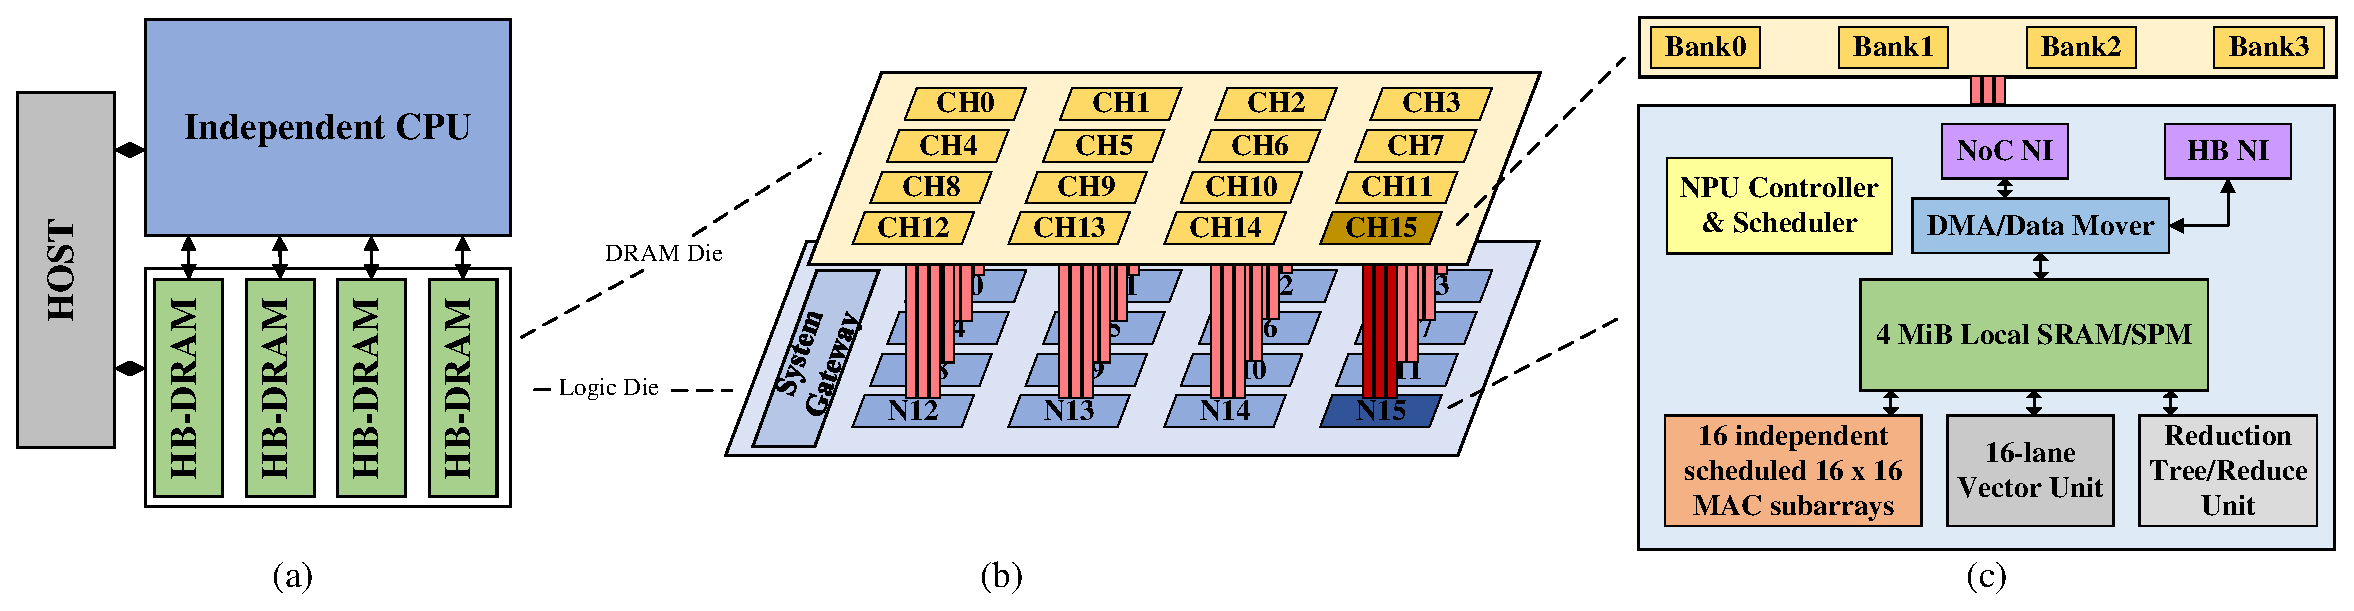
\includegraphics[width=\columnwidth]{figures/target_architecture.pdf}
  \caption{Target 3D system. (a) Host and HB-DRAM organization. (b) Face-to-face
  integration of the $4\times4$ Logic-tier NPU mesh and the aligned DRAM
  channels. (c) Microarchitecture of an NPU--memory pair.}
  \Description{Three panels show the host and HB-DRAM organization, the
  vertically aligned NPU clusters and DRAM channels, and the internal
  organization of one NPU--memory pair.}
  \label{fig:target-architecture}
\end{figure}

Figure~\ref{fig:target-architecture} shows a 3D accelerator in which the
logic and memory tiers are integrated by face-to-face hybrid bonding.
Each NPU cluster in the logic tier is vertically aligned with a DRAM
partition and accesses it through a local hybrid-bond link. A baseline
horizontal $4\times4$ Mesh NoC connects the NPU clusters and carries
inter-cluster transfers, including MoE Dispatch and Combine traffic.
Local memory accesses and inter-cluster transfers therefore use distinct
physical paths. The stacked logic and DRAM dies are thermally coupled,
imposing a peak-temperature constraint on execution.

To study co-execution, we replay an MoE dispatch trace alongside synthetic
cache-coherence read requests that represent general-purpose memory traffic.
The requests and their responses traverse the same horizontal mesh as the
MoE traffic.

The main MoE evaluation covers Qwen3-30B-A3B~\cite{qwen3report} and
Qwen1.5-MoE-A2.7B~\cite{qwen15moe} for language-model inference,
mini-SWE-agent~\cite{minisweagent} with a Qwen3-30B-A3B backend for
SWE-bench Lite tasks~\cite{swebench}, and LingBot TI2V~\cite{lingbotvideo}
for video generation. The auxiliary thermal scenario combines
WHISPER~\cite{whisper}, an ORB-SLAM3-derived SLAM workload~\cite{orbslam3},
and $\pi_{0.5}$~\cite{pi05}.


\subsection{Phase-Dependent Congestion in MoE Communication}

\noindent\textbf{Problem.}
HiBand adapts communication locality by switching among four topologies---
Full-Local, Local-Biased, Global-Biased, and Full-Global---that repartition
bandwidth according to broad communication locality~\cite{wang2026hiband}.
MoE communication can concentrate transfers around a small set of busy NPU
nodes and links. When several messages need the same link or router output,
they must wait even if other parts of the network have spare capacity.
As hotspot locations change, the four predefined topologies may still leave
concentrated flows competing for the same links and router outputs, causing
persistent queueing despite spare capacity elsewhere.

Figure~\ref{fig:noc-phenomenon}(a) shows the communication latency of
Qwen3-30B-A3B prefill. As input length increases
from 128 to 1024 tokens per request, the queueing share of mean network
round-trip latency rises from 57.2\% to 88.8\%, while mean zero-load latency
increases by 17.3\%. Zero-load latency includes serialization and traversal
without competing traffic; queueing is the additional delay under concurrent
traffic. Thus, queueing at shared network resources dominates the growth in
communication latency as input length increases.

\noindent\textbf{Root Cause.}
The gating network (Gate) selects a small set of experts for each token.
During Dispatch, token activations are sent to the NPU nodes holding those
experts; Combine returns the corresponding expert outputs. We define a flow
as the messages from one source NPU to one destination NPU within a single
communication phase. During Dispatch, when many tokens select the same experts, or several
frequently selected experts reside on the same NPU, transfers concentrate at
a small set of destinations. Flows whose routes overlap then compete for
shared links and router outputs, creating queueing hotspots. Thus, hotspot
formation depends on both the distribution of Gate selections and expert placement.
Our controlled Qwen3 decoding test also shows that concentrated accesses
can serialize requests at shared DRAM banks. Spreading those accesses across
banks addresses memory-side waiting, while overlapping NoC routes still
require path-level control.

Figure~\ref{fig:noc-phenomenon}(b) maps these messages onto deterministic XY paths.
Across MoE model layers 1, 24, and 48, the largest path-derived router demand
occurs at R9, R5, and R10, respectively. This spatial concentration can force multiple flows to share a
router output or link. Different concentrations can require different local
connections even when their total volume and aggregate communication locality
are similar. The design requirement is therefore to provide selectable local
paths around the contested resources, with explicit capacity at their
injection and receiving interfaces.

Even short cache-coherence read requests can add substantial load when
they arrive frequently. When they share a router output with an MoE
dispatch burst, queueing can delay their responses. In our replay,
staggering the two streams restores the latency of the step waiting for
coherence responses to the coherence-only level.

\begin{figure*}[!t]
  \centering
  \begin{minipage}[t]{0.36\textwidth}
    \vspace{0pt}\centering
    {\small (a) Prefill latency\par}
    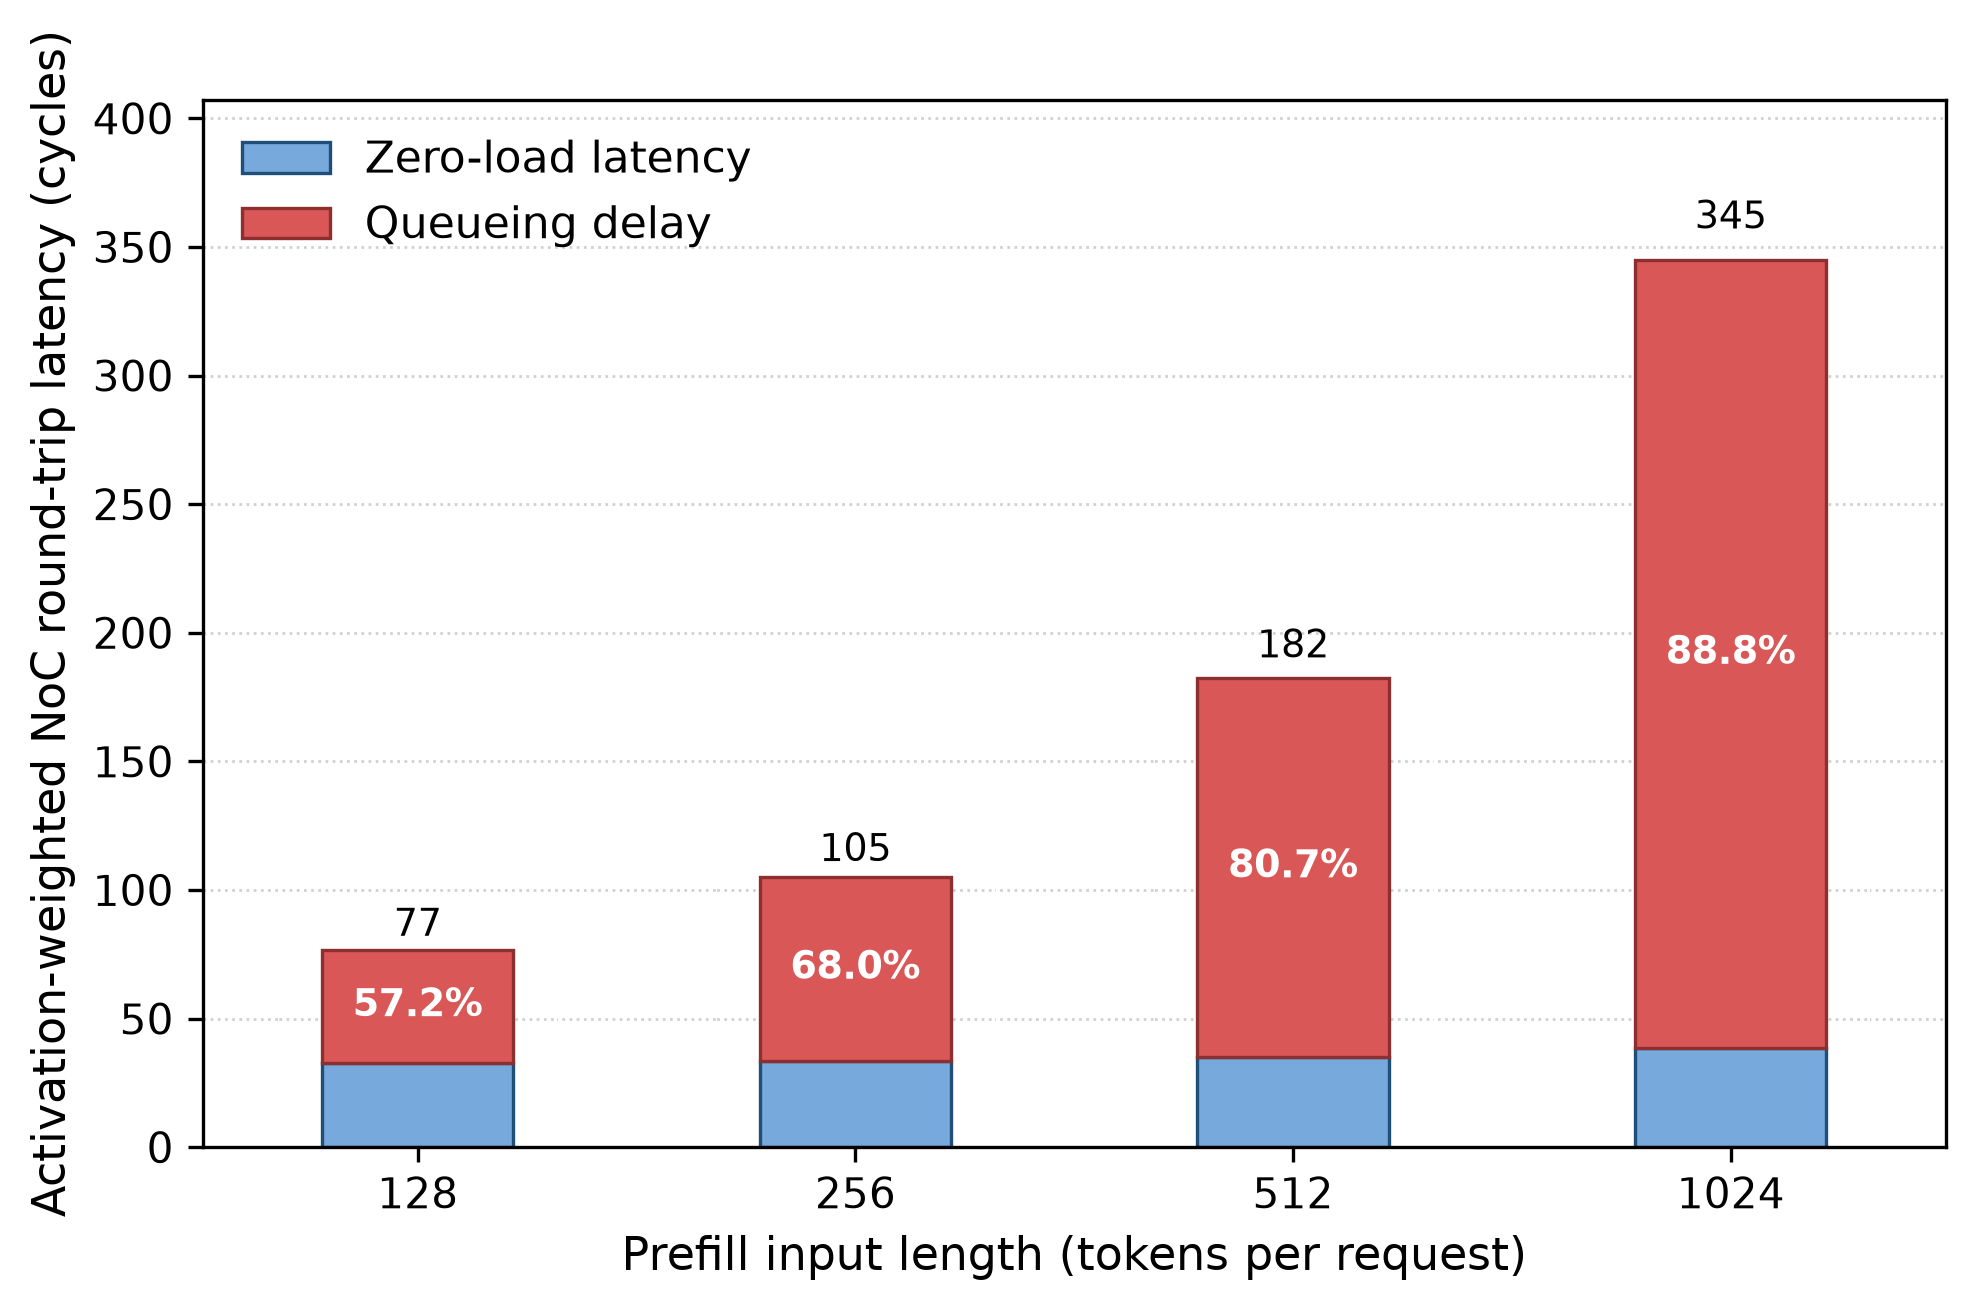
\includegraphics[width=\linewidth]{figures/noc_phenomenon_narrow_bars.png}
  \end{minipage}\hfill
  \begin{minipage}[t]{0.62\textwidth}
    \vspace{0pt}\centering
    {\small (b) Router demand across MoE layers\par}
    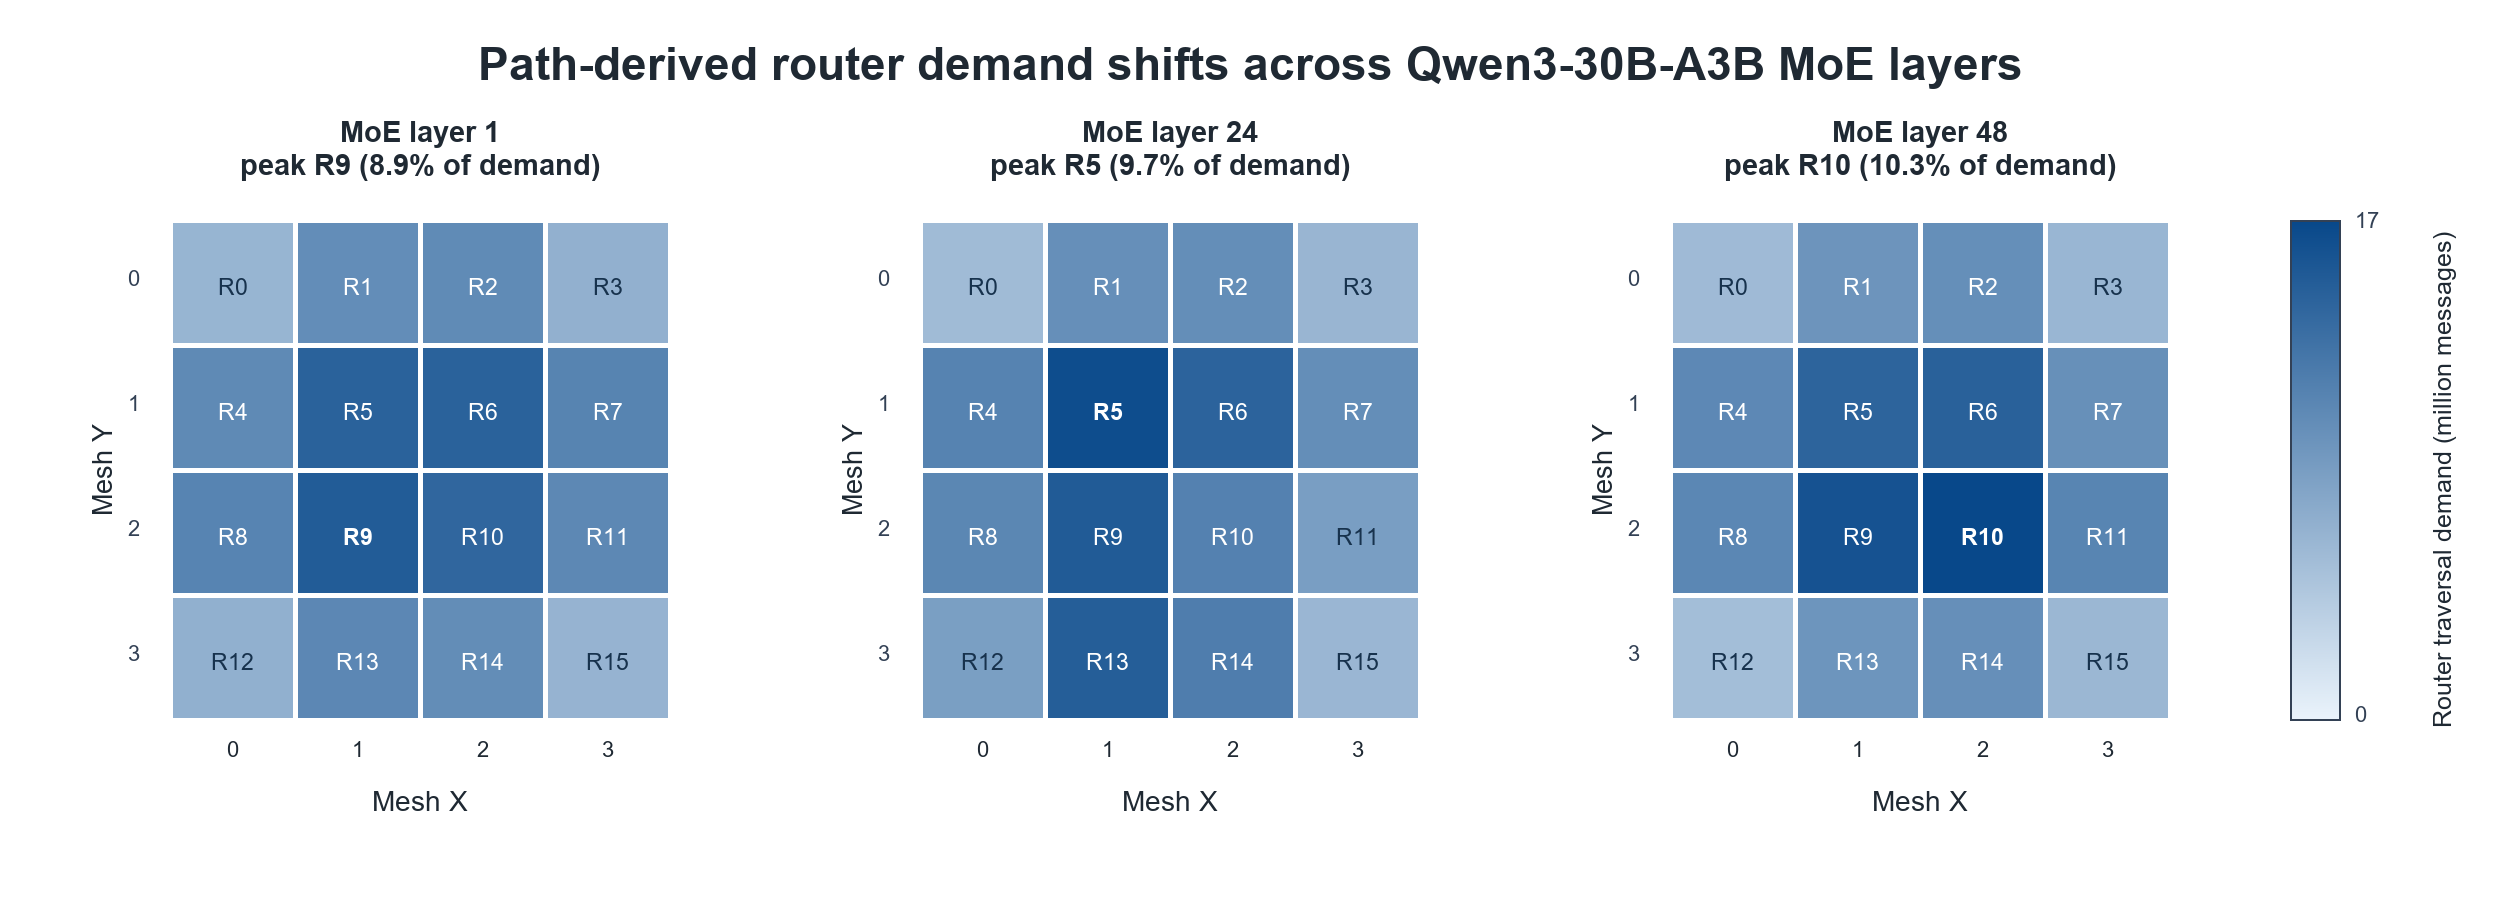
\includegraphics[width=\linewidth,trim=0bp 0bp 0bp 24bp,clip]{figures/noc_cause_router_hotspots_revised.png}
  \end{minipage}
  \caption{Communication latency and router demand for Qwen3-30B-A3B.
  (a) Activation-weighted mean NoC round-trip latency on the fixed Mesh.
  The queueing share rises from 57.2\% to 88.8\% as prefill input grows
  from 128 to 1024 tokens.
  (b) Router demand along deterministic XY paths on a shared color scale.
  The peak moves from R9 to R5 to R10 across MoE layers 1, 24, and 48.}
  \Description{Four stacked bars show the growth in queueing delay with
  input length. Three heatmaps show the change in peak router demand
  across MoE layers.}
  \label{fig:noc-phenomenon}
\end{figure*}

\noindent\textbf{Opportunity: Configurable Connections.}
Configurable paths can provide additional channels for heavy transfers and
reduce intermediate-router forwarding. Figures~\ref{fig:noc-opportunity}(a) and (b)
illustrate these opportunities using three transfers. For neighboring
nodes, the $\mathrm{NI}_5$--$\mathrm{CS}_1$--$\mathrm{NI}_6$ circuit adds
a channel alongside the existing Mesh link. A separate
$\mathrm{NI}_5$--$\mathrm{CS}_3$--$\mathrm{NI}_9$ circuit allows the same
source to communicate with another peer without sending both transfers
through its local Mesh router. For the distant $N_0$-to-$N_{15}$ transfer,
interconnected lower and upper CSs form an NI-to-NI path that bypasses
intermediate Mesh routers. These connections can be reassigned between
communication phases to serve changing peers and heavy source--destination
pairs. Thus, the same physical network supports additional neighboring-node
bandwidth, communication with multiple peers, and router bypass for distant
transfers, subject to the shared service capacities of the NIs, DMA engines,
and SRAM banks.

Arbitration allocates transmission opportunities on the shared output.
Round-robin and priority arbitration cannot prevent queue buildup when
aggregate demand persistently exceeds the output's service capacity.
In Fig.~\ref{fig:noc-opportunity}(c), routing the selected MoE packet
through CS3 from NI4 to NI8 removes its contention with coherence reads
at the N4-to-N8 mesh output. We assess the benefit by when the step that
requires both branches becomes ready.

\begin{figure*}[!t]
  \centering
  \begin{minipage}[t]{0.49\textwidth}
    \vspace{0pt}\centering
    {\small (a) Ordinary Mesh paths\par}
    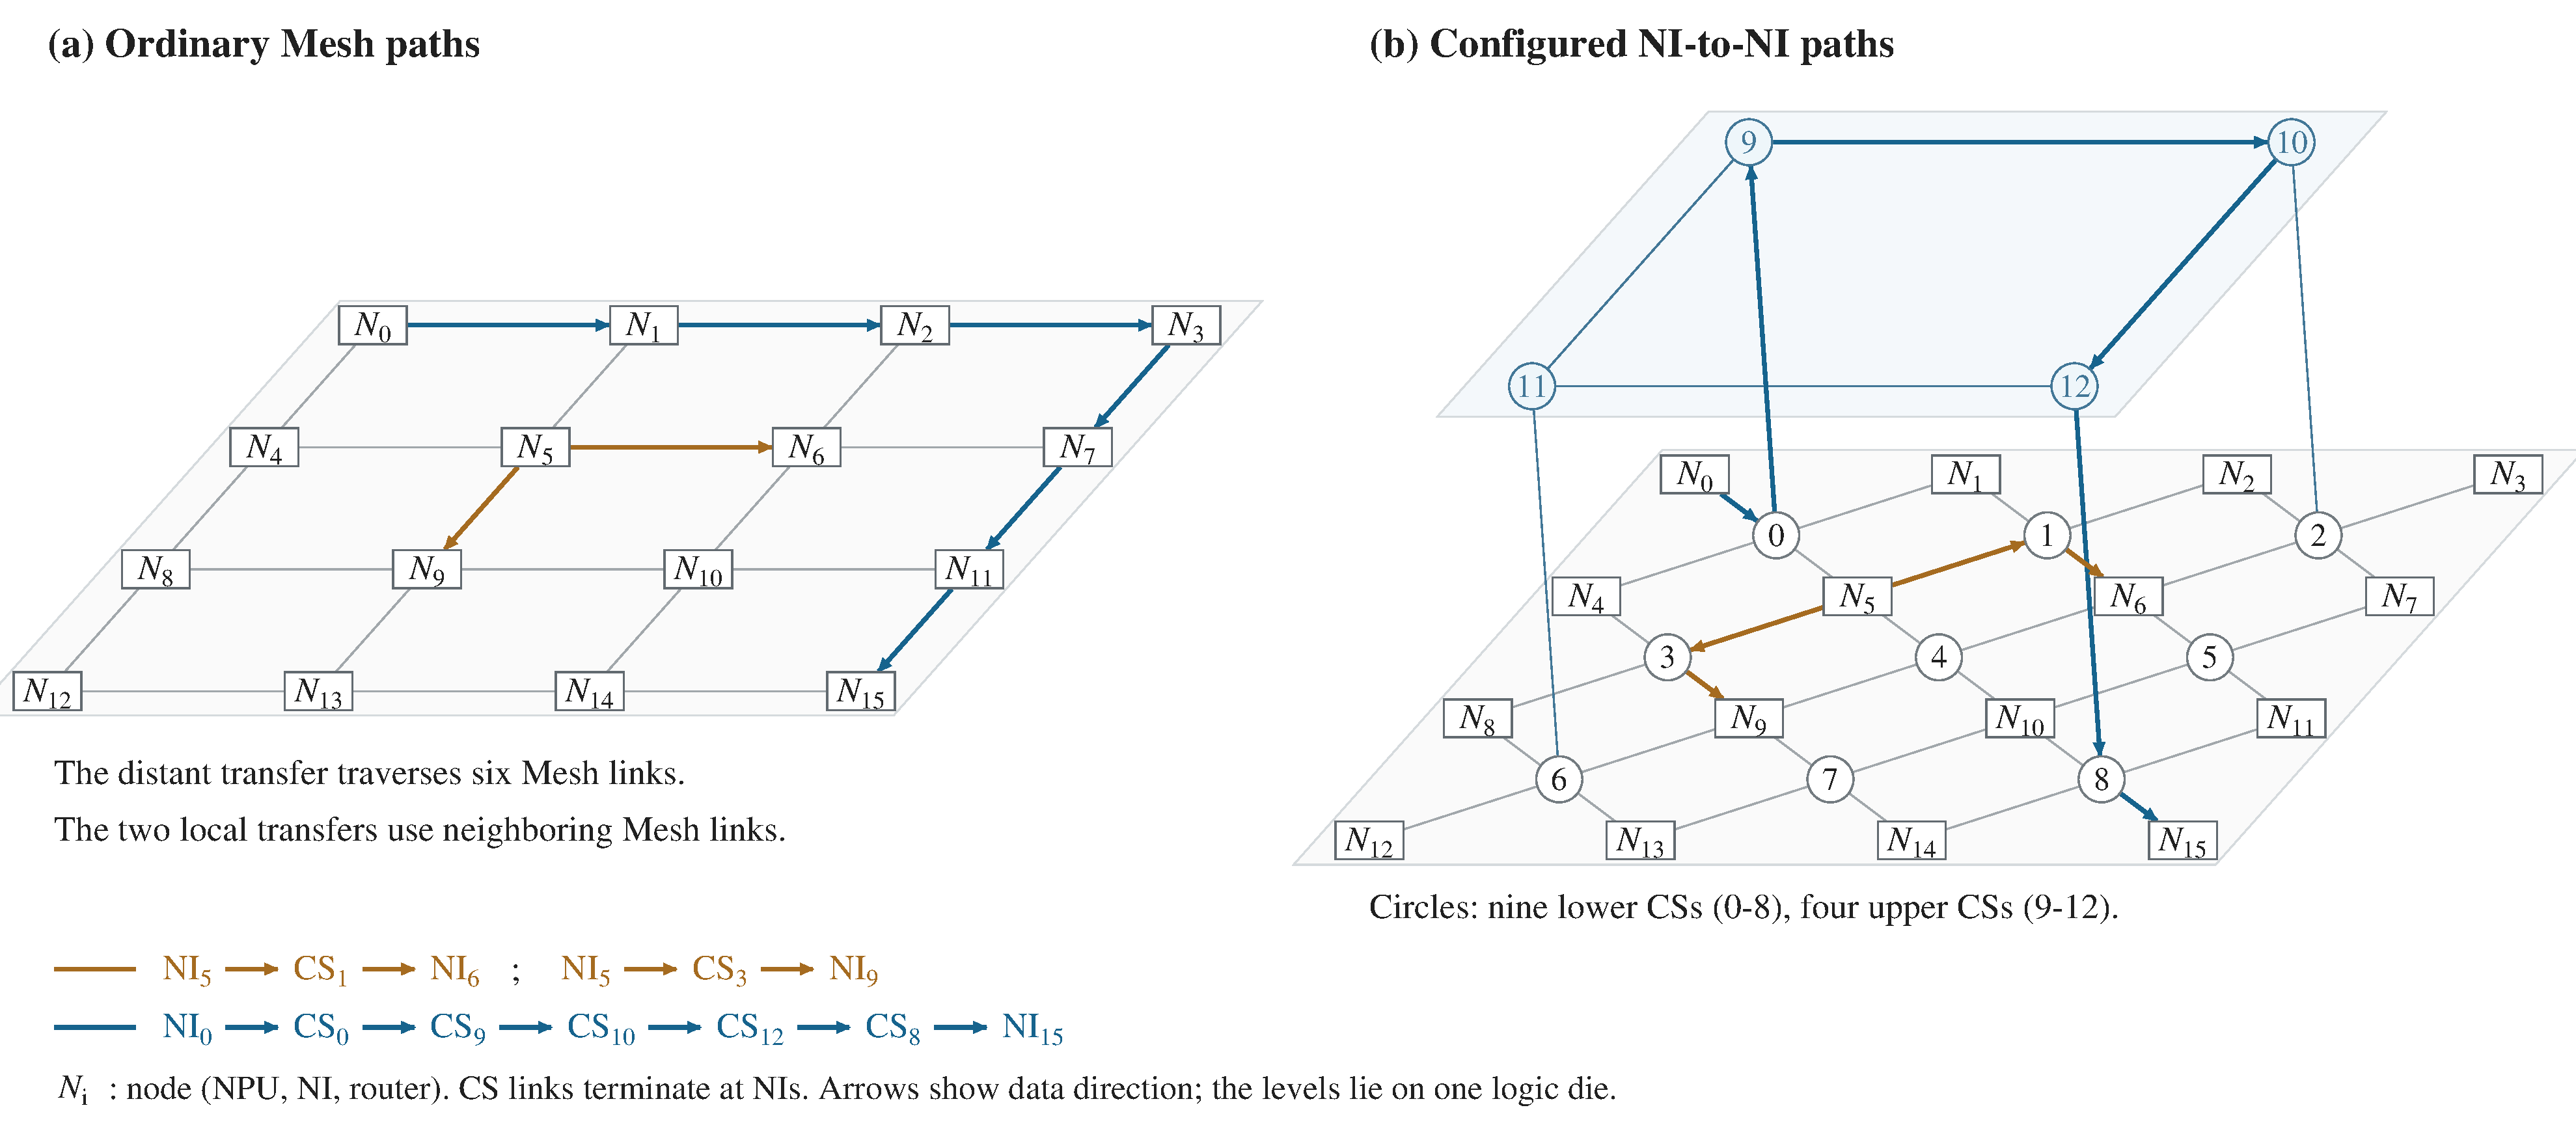
\includegraphics[width=\linewidth,trim=0bp 201bp 950bp 214bp,clip]{figures/noc_opportunity_current.pdf}\par
    \vspace{3pt}
    {\small (c) Co-execution timing\par}
    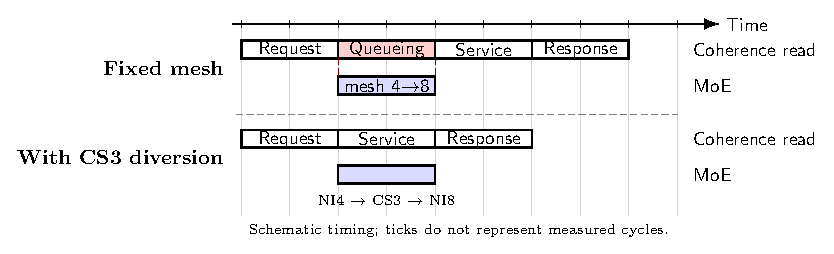
\includegraphics[width=\linewidth]{figures/figure3_contention.pdf}\par
  \end{minipage}\hfill
  \begin{minipage}[t]{0.49\textwidth}
    \vspace{0pt}\centering
    {\small (b) Configured NI-to-NI paths\par}
    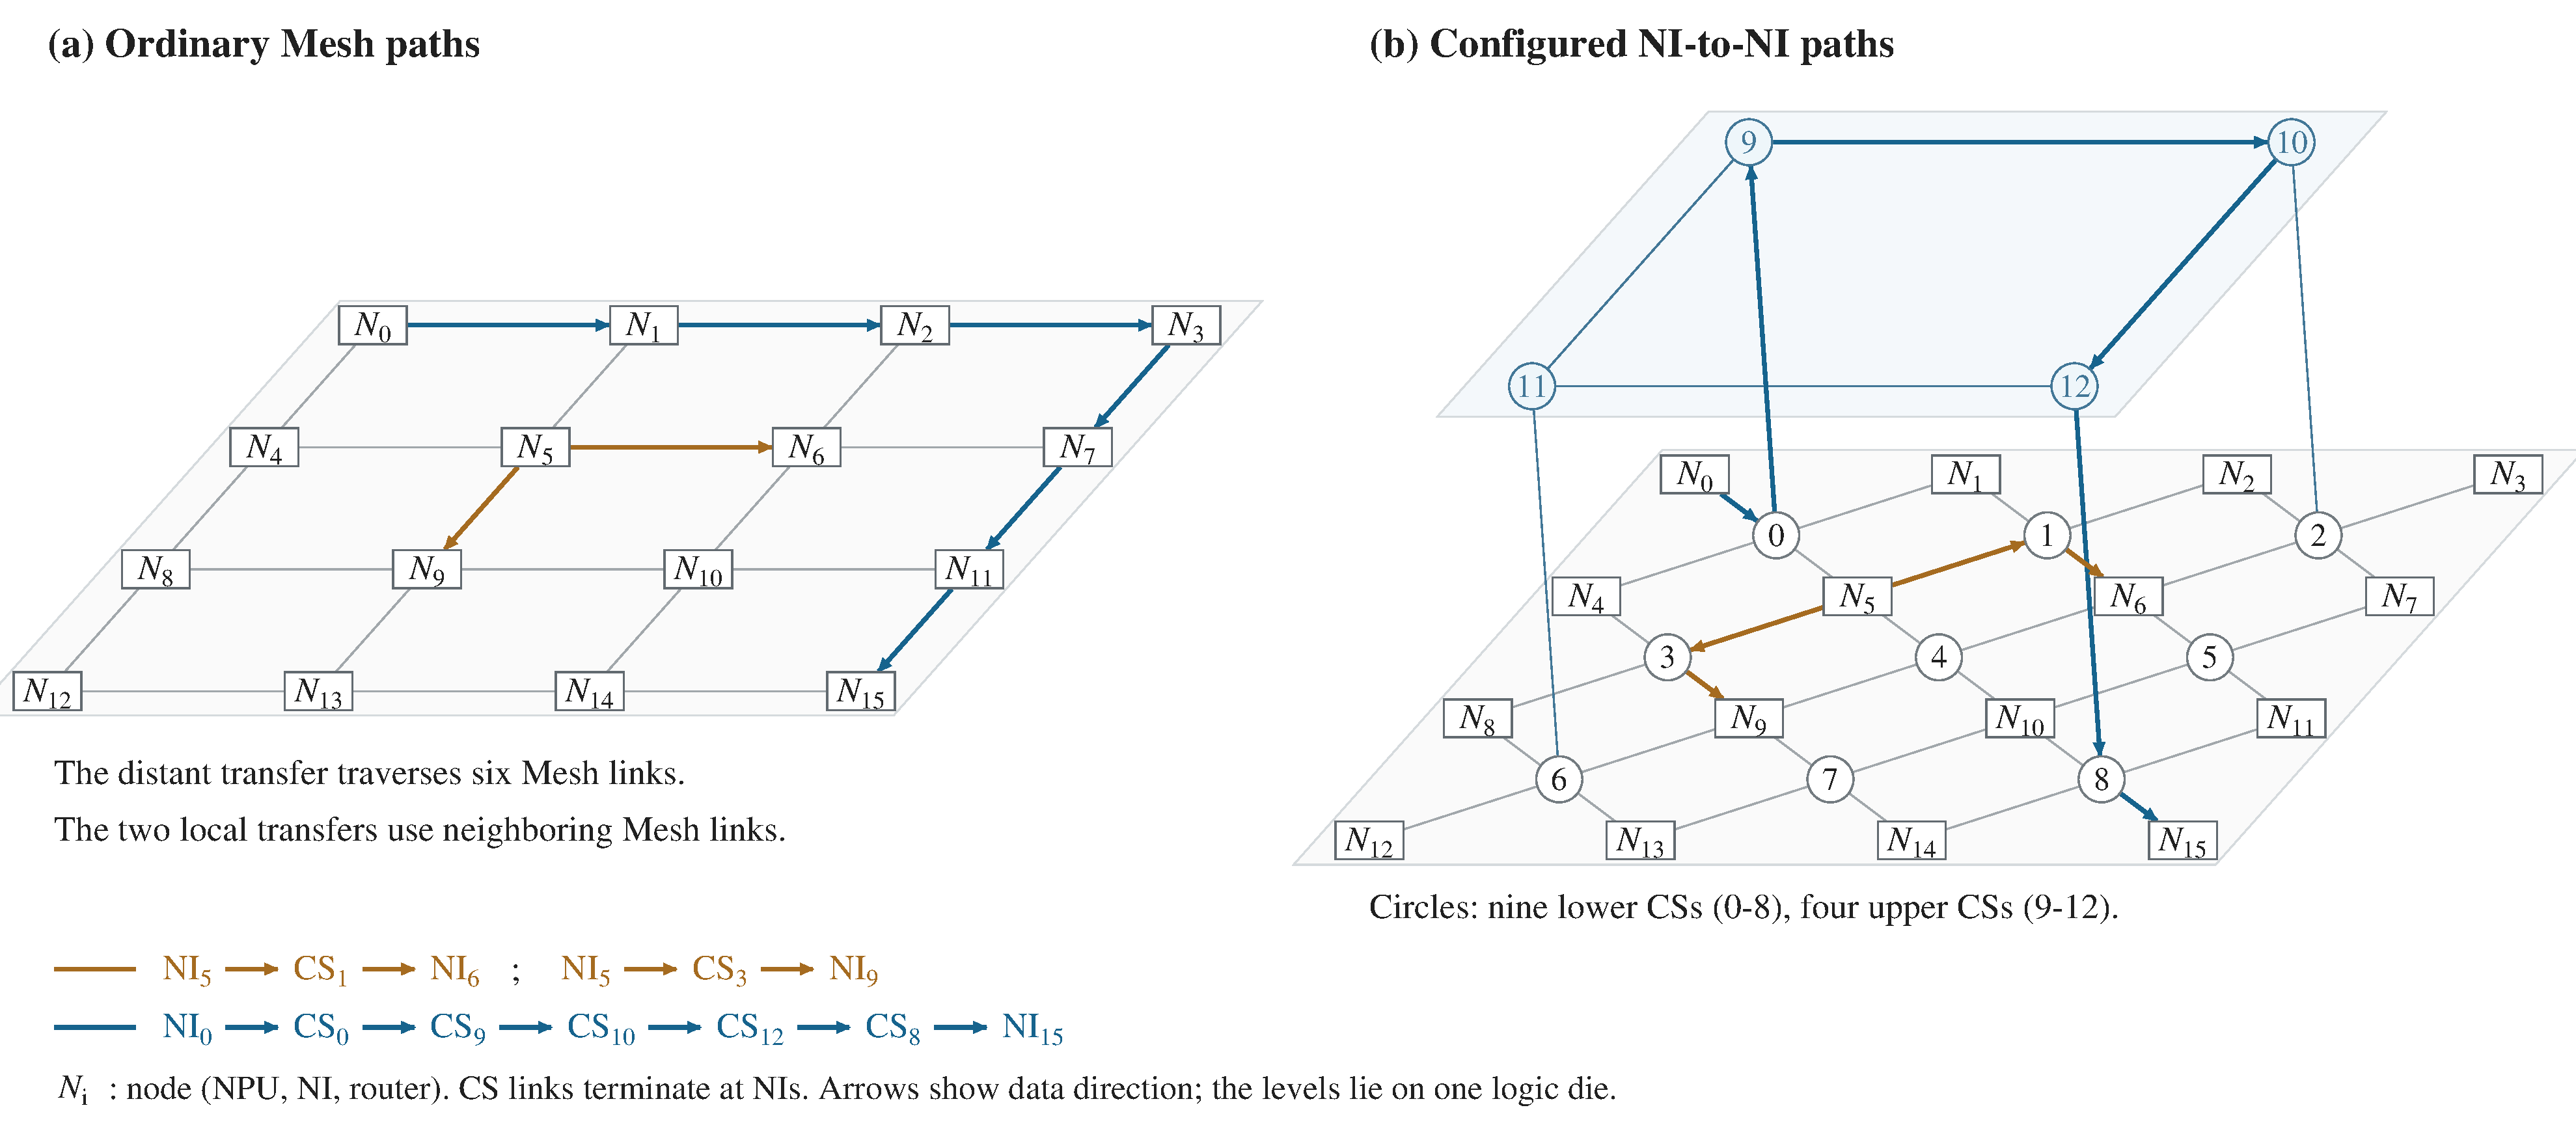
\includegraphics[width=\linewidth,trim=950bp 145bp 0bp 62bp,clip]{figures/noc_opportunity_current.pdf}\par
    \vspace{2pt}
    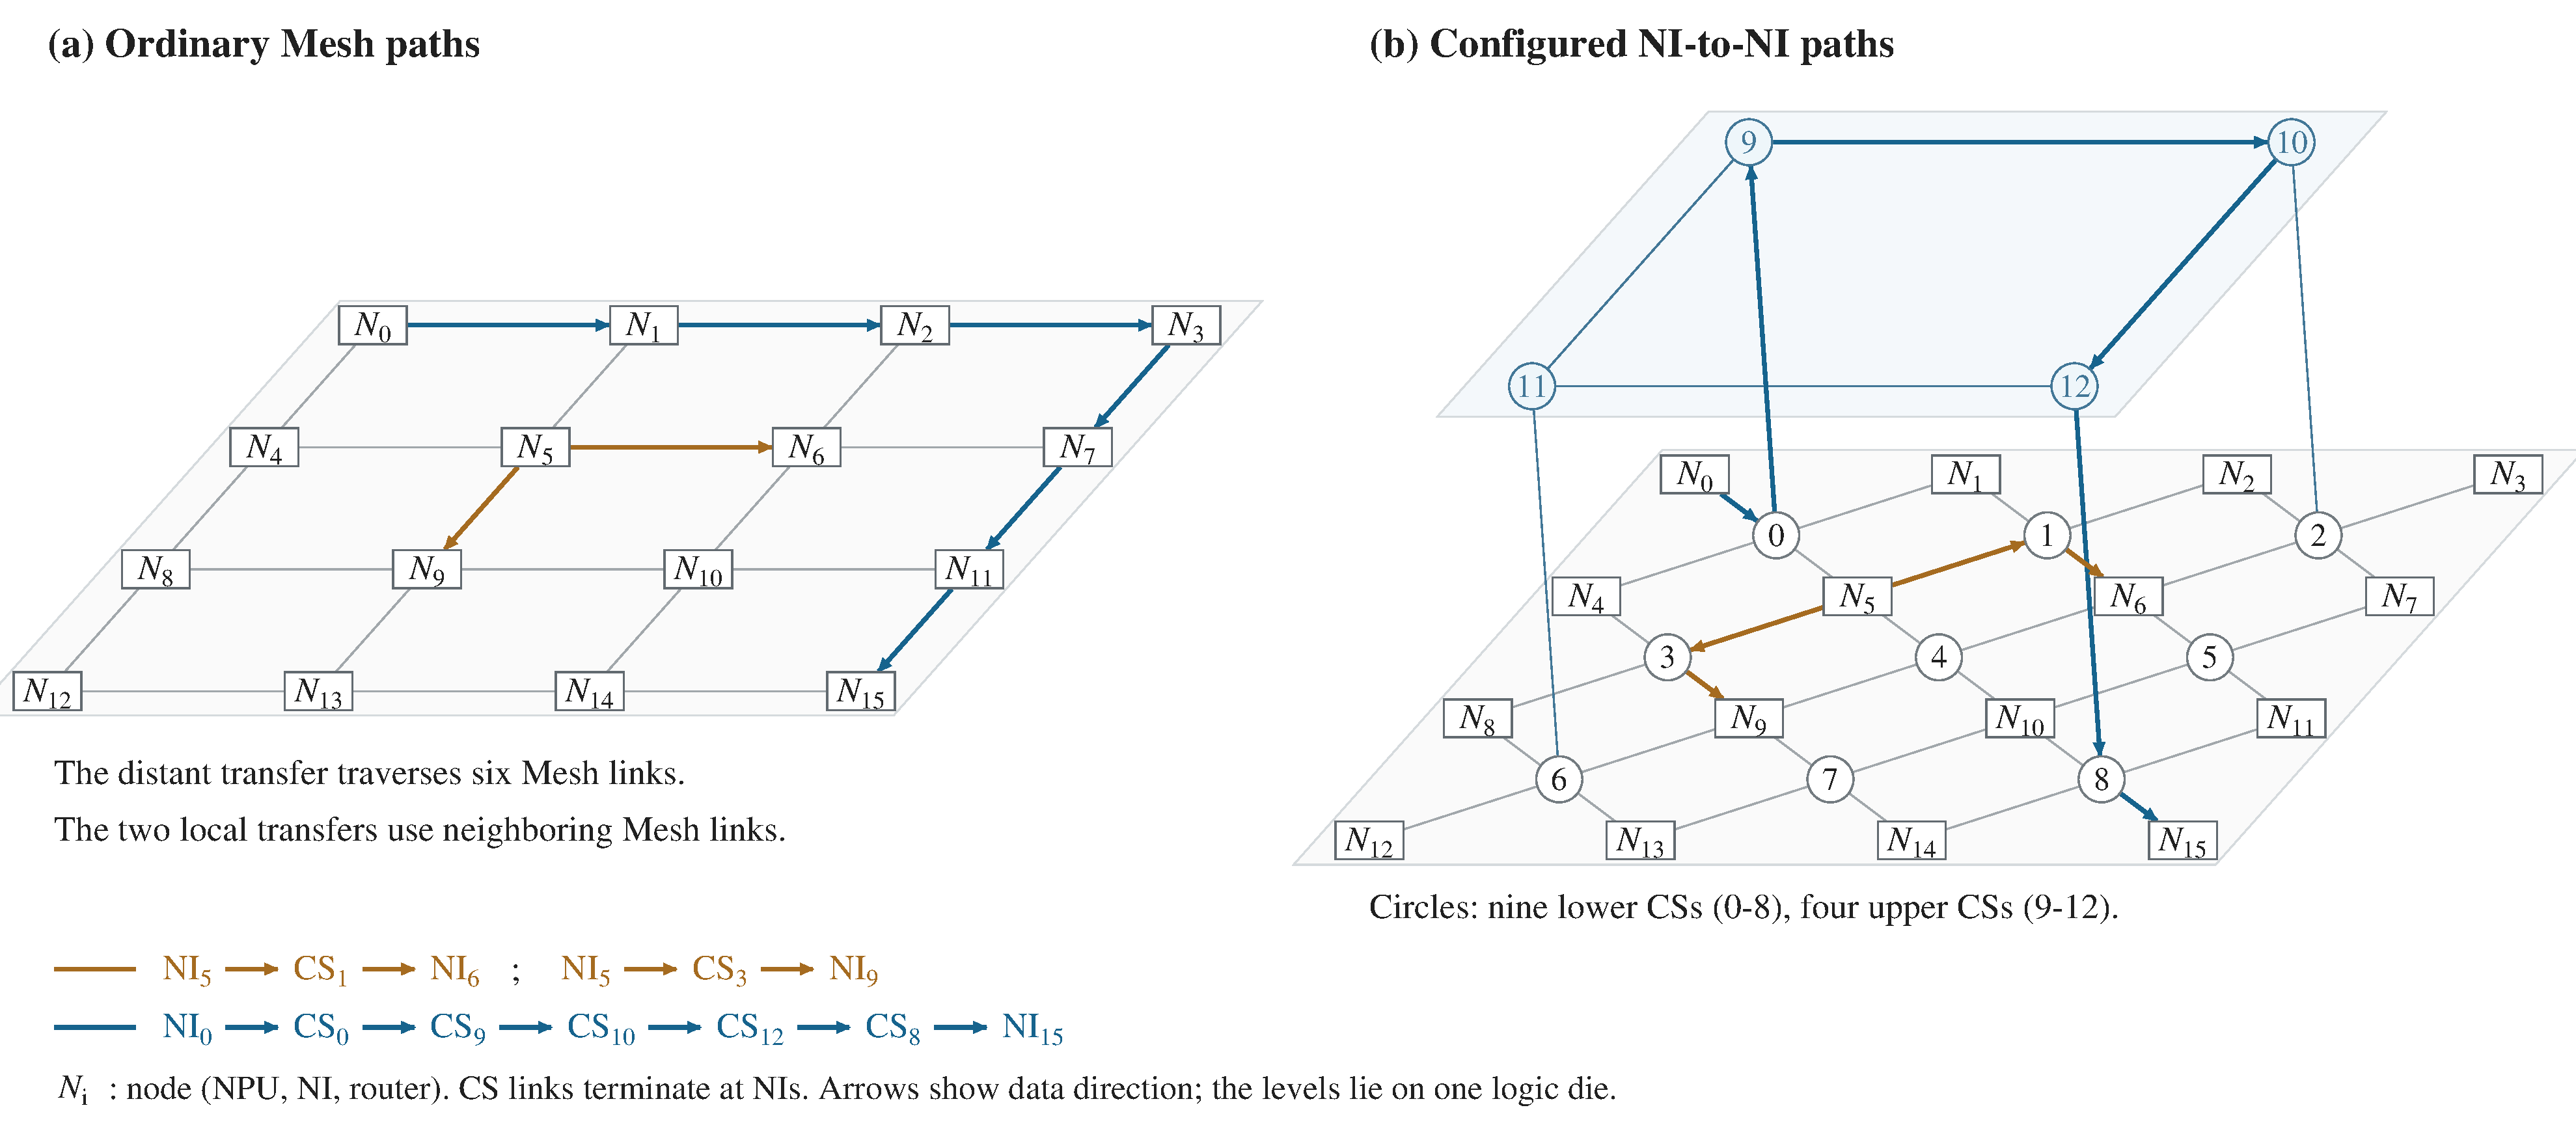
\includegraphics[width=\linewidth,trim=0bp 0bp 680bp 686bp,clip]{figures/noc_opportunity_current.pdf}
  \end{minipage}
  \caption{Configurable paths for co-execution. (a) Ordinary Mesh routes.
  (b) Local and cross-region circuits. (c) Illustrative timing of CS3
  diversion around the shared $N_4$-to-$N_8$ Mesh output.}
  \Description{Three panels show the ordinary Mesh paths, three circuits
  through the configurable-switch network, and timing diagrams comparing
  queueing on the fixed Mesh with CS3 diversion.}
  \label{fig:noc-opportunity}
\end{figure*}


\noindent\textbf{Thermal Management.}
Concentrated activity in the stacked Logic and DRAM tiers raises temperatures in both tiers, increasing the risk of thermal throttling, which can increase inference latency. While task migration has been widely studied for thermal management, its effectiveness in DRAM-stacked NPUs is limited by the strong dependence of computation on locally stored model weights. Migrating tasks may require weight replication or remote memory accesses, introducing additional DRAM and NoC overhead. Our experiments show that these costs largely offset the performance benefits of task migration. Therefore, instead of relocating tasks, we reduce heat generation through operator-level energy-aware DVFS and improve execution efficiency through thermal-aware task scheduling.

\section{Design}
\label{sec:design}

\subsection{Reconfigurable Network}
\label{sec:noc-design}

Figure~\ref{fig:noc-physical-design}(a) shows the reconfigurable network
alongside the basic $4\times4$ Mesh. The logic tier contains sixteen NPU
nodes, nine lower-level configurable switches (CSs), and four upper-level
CSs. Nodes $N_0$--$N_{15}$ and lower CSs $\mathrm{CS}_0$--$\mathrm{CS}_8$
are indexed in row-major order. Each lower CS physically connects to
the NIs of the four corner nodes of a $2\times2$ group. A corner, edge, or interior node
therefore connects to one, two, or four lower CSs, respectively.
The upper CSs form a $2\times2$ network:
$\mathrm{CS}_9$, $\mathrm{CS}_{10}$, $\mathrm{CS}_{11}$, and
$\mathrm{CS}_{12}$ connect down to $\mathrm{CS}_0$, $\mathrm{CS}_2$,
$\mathrm{CS}_6$, and $\mathrm{CS}_8$, respectively.
Each upper CS connects to its corresponding lower CS and two upper
neighbors. For a local transfer, a lower CS selects one node-facing
input and a different node-facing output. A connection between a node
and the upper network instead selects one node-facing direction and U.
The upper network provides additional paths between the four lower
CSs attached to it. Upper CSs reach NPU nodes through these lower CSs.
The two CS levels are connectivity levels within the same logic die.
Their MUXes, configuration registers, and control gates are implemented
as logic cells, with the connections routed in the die's metal stack.
The separated planes in the figure depict this connectivity hierarchy.

Figure~\ref{fig:noc-physical-design}(b) shows the two CS circuits.
A lower CS has four corner directions, northwest (NW), northeast (NE),
southwest (SW), and southeast (SE), and an upper direction U.
Only the four lower CSs listed above have a physical U attachment.
In the other five instances, the U input data and valid signals are
tied to zero, the U output enable is hardwired to zero, and the
U-side ready input is tied to zero. These constant connections are
fixed at implementation time and cannot be changed by configuration
writes. Figure~\ref{fig:noc-physical-design}(b) depicts the lower-CS
circuit with a connected U direction. An upper CS has two in-plane
directions and a downward direction D. The lower and upper circuits
use five 4:1 multiplexers (MUXes) and three 2:1 MUXes, respectively.
Each output MUX is wired to the other directions' inputs, excluding
a return to its own direction. The configuration register supplies
an output-direction code, an input-selection code, and a connection
enable (EN). Direction decoding enables at most one output, so each
CS establishes at most one directed input--output connection.

A short transfer between two nodes attached to the same lower CS can
use that CS directly between its source and destination NIs.
This circuit provides an additional data channel alongside the Mesh,
increasing the available path bandwidth and moving part of the traffic
away from contended Mesh links and router outputs. Circuits through the
upper network connect nodes attached to different U-connected lower
CSs, bypassing intermediate Mesh routers.
Multiple CS attachments allow a node to participate in separate circuits.
A heavily communicating neighboring pair can use an additional CS path
alongside its Mesh connection. These connections can be reassigned as the
busy endpoints and node pairs change between communication phases.
Traffic without an assigned circuit uses the ordinary Mesh.
The aggregate transfer rate is also limited by NI service and SRAM
bank bandwidth.

\begin{figure*}[!t]
  \centering
  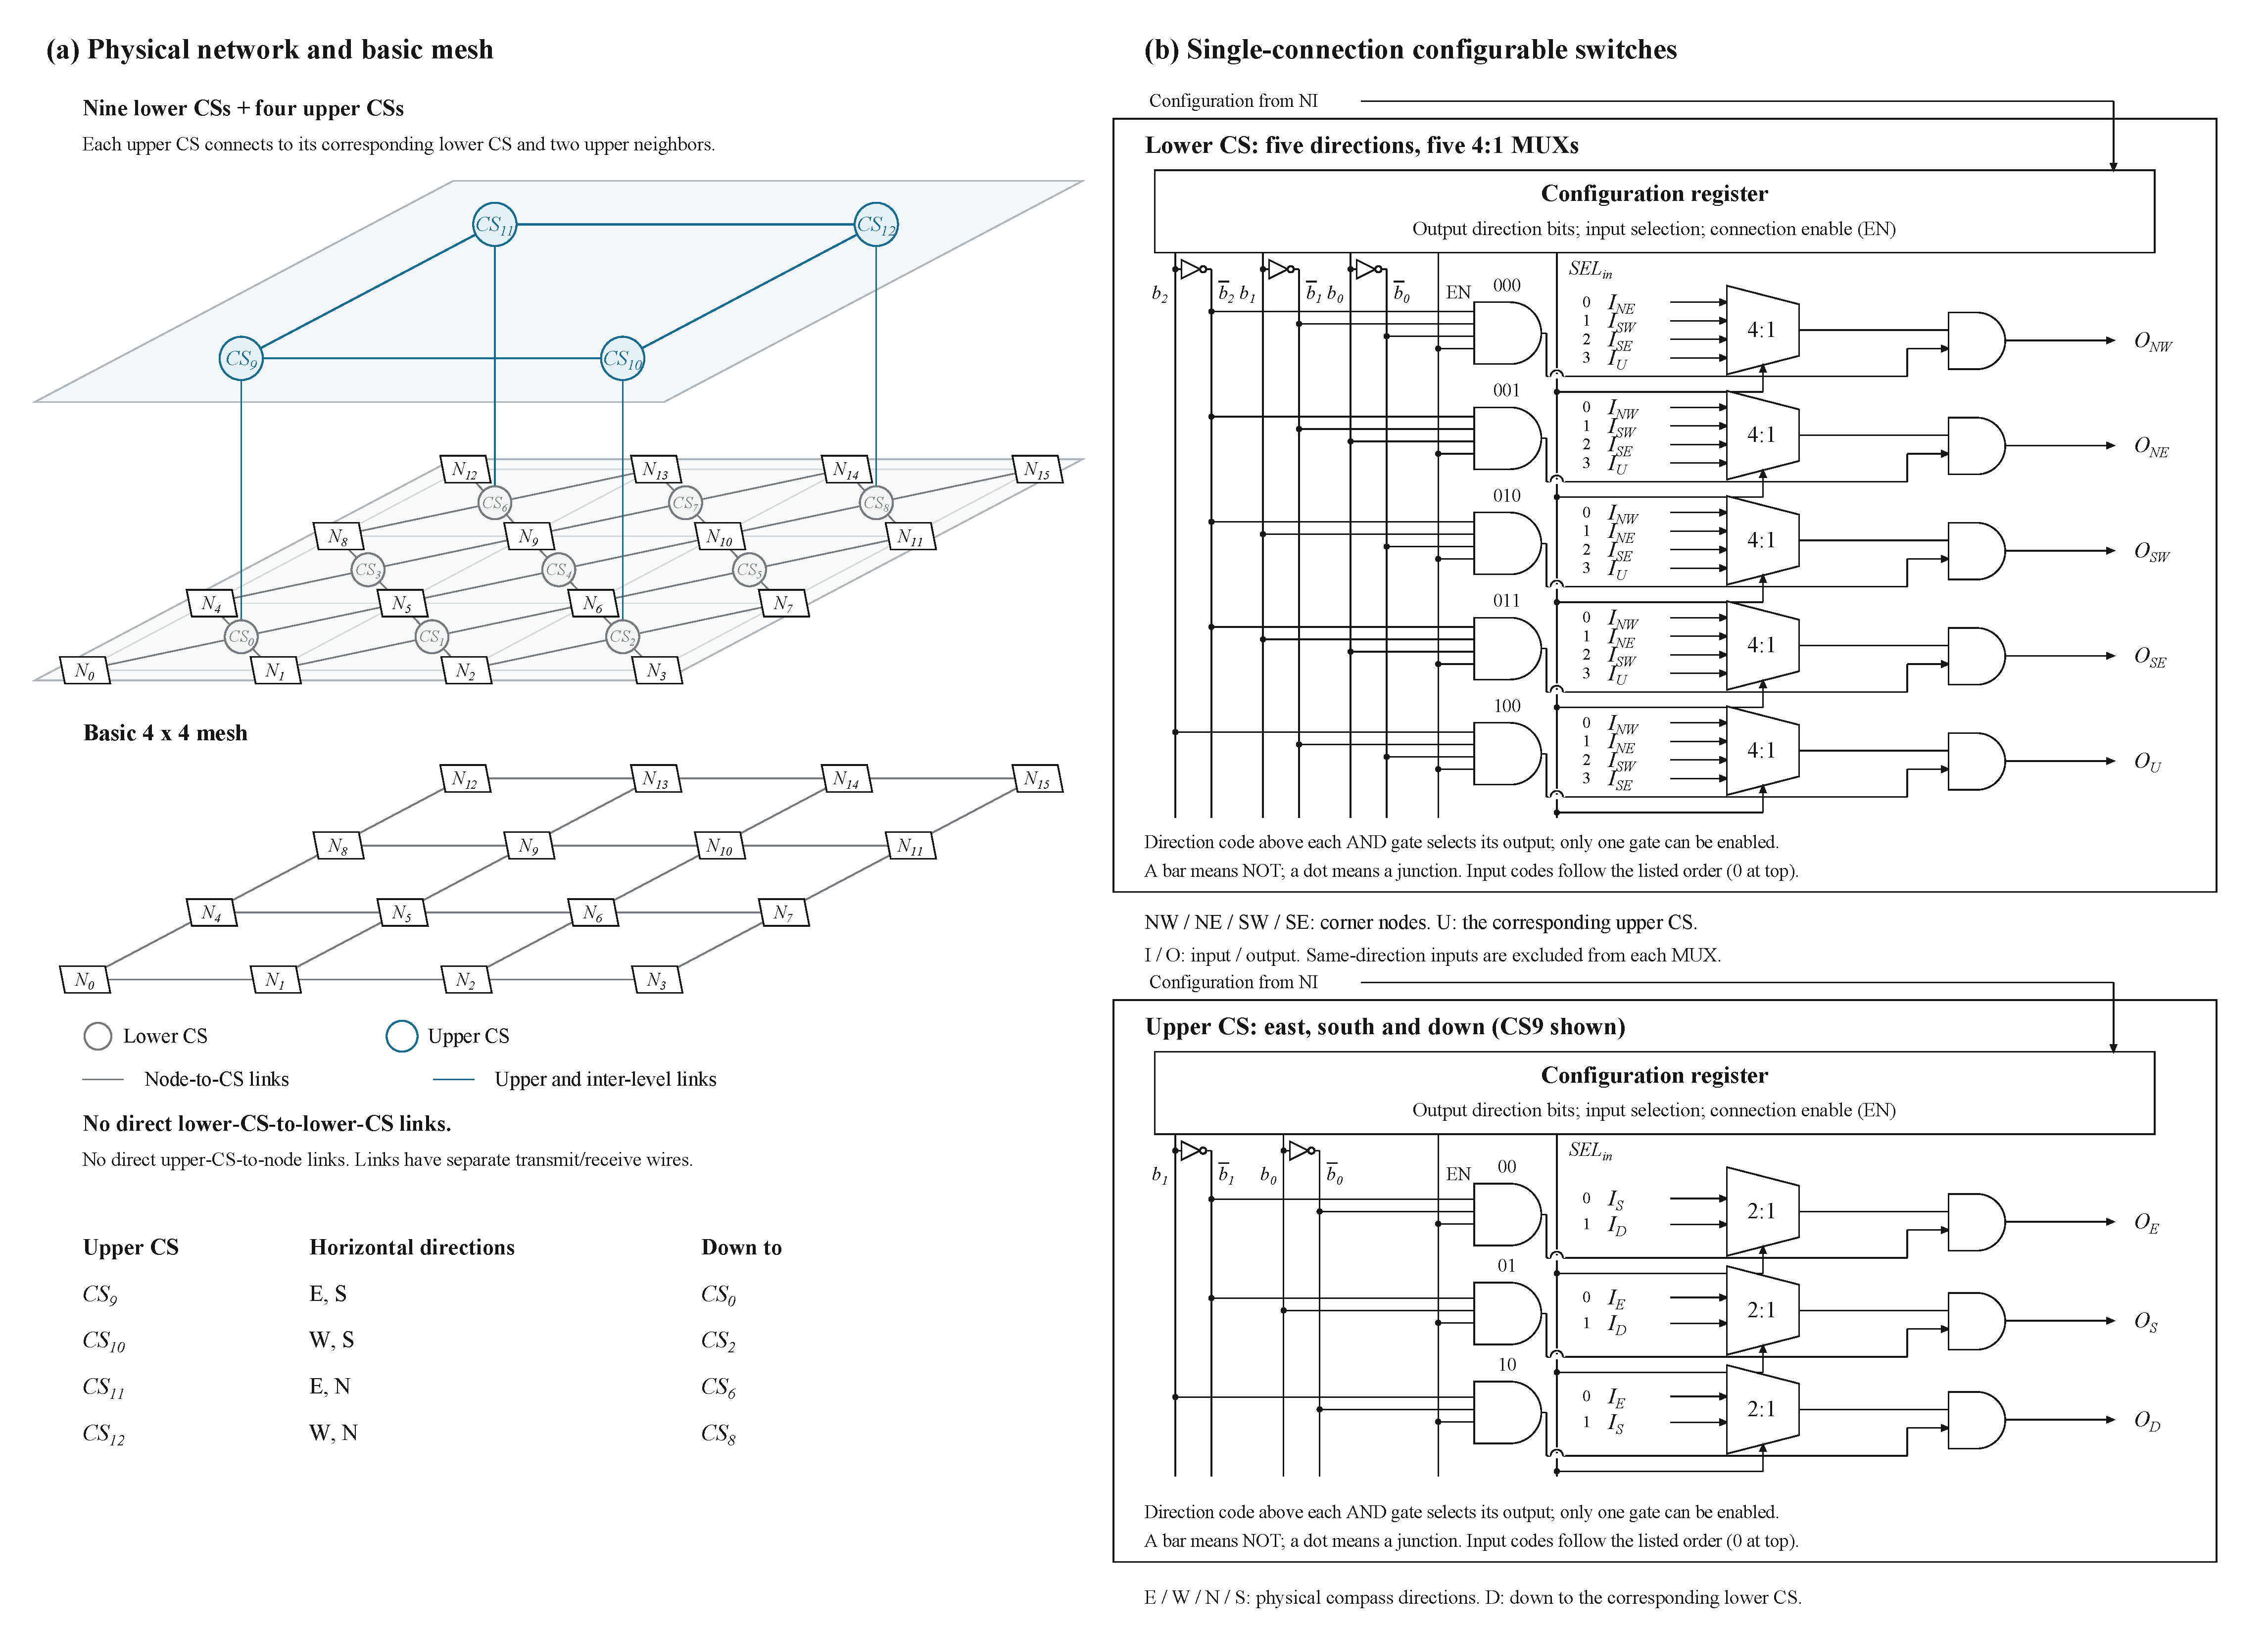
\includegraphics[width=\textwidth]{figures/noc_topology_cs.pdf}
  \caption{Reconfigurable network and switch circuits.
  (a) Nine lower CSs and four interconnected upper CSs, with the basic
  Mesh shown for comparison. The separated planes denote connectivity
  levels on one logic die. (b) A U-connected lower CS and an upper CS.
  Each MUX excludes its own direction's input; output decoding enables
  one connection.}
  \Description{The left panel shows the two levels of configurable switches
  and a basic Mesh. Only four lower switches attach to upper switches.
  The right panel expands the five-direction lower switch and
  three-direction upper switch, including configuration registers,
  direction decoding, input MUXes, and output enable gates.}
  \label{fig:noc-physical-design}
\end{figure*}

\subsection{Node and Network Interface}
\label{sec:noc-node-design}

Figure~\ref{fig:noc-node}(a) expands an NPU node. Its NPU cluster contains
a multiply--accumulate (MAC) array and a vector unit. A banked SRAM
scratchpad holds local weights and activations. The SRAM access controller
arbitrates bank requests from the NPU and the network interface (NI).
The Mesh router retains its four directional connections and a local
NI connection. The NI also has separate transmit and receive connections
to each adjacent lower CS. NW, NE, SW, and SE beneath the CSs in this
figure identify their positions relative to the node; a CS northwest
of the node uses its own SE direction to reach that node.

\begin{figure*}[!t]
  \centering
  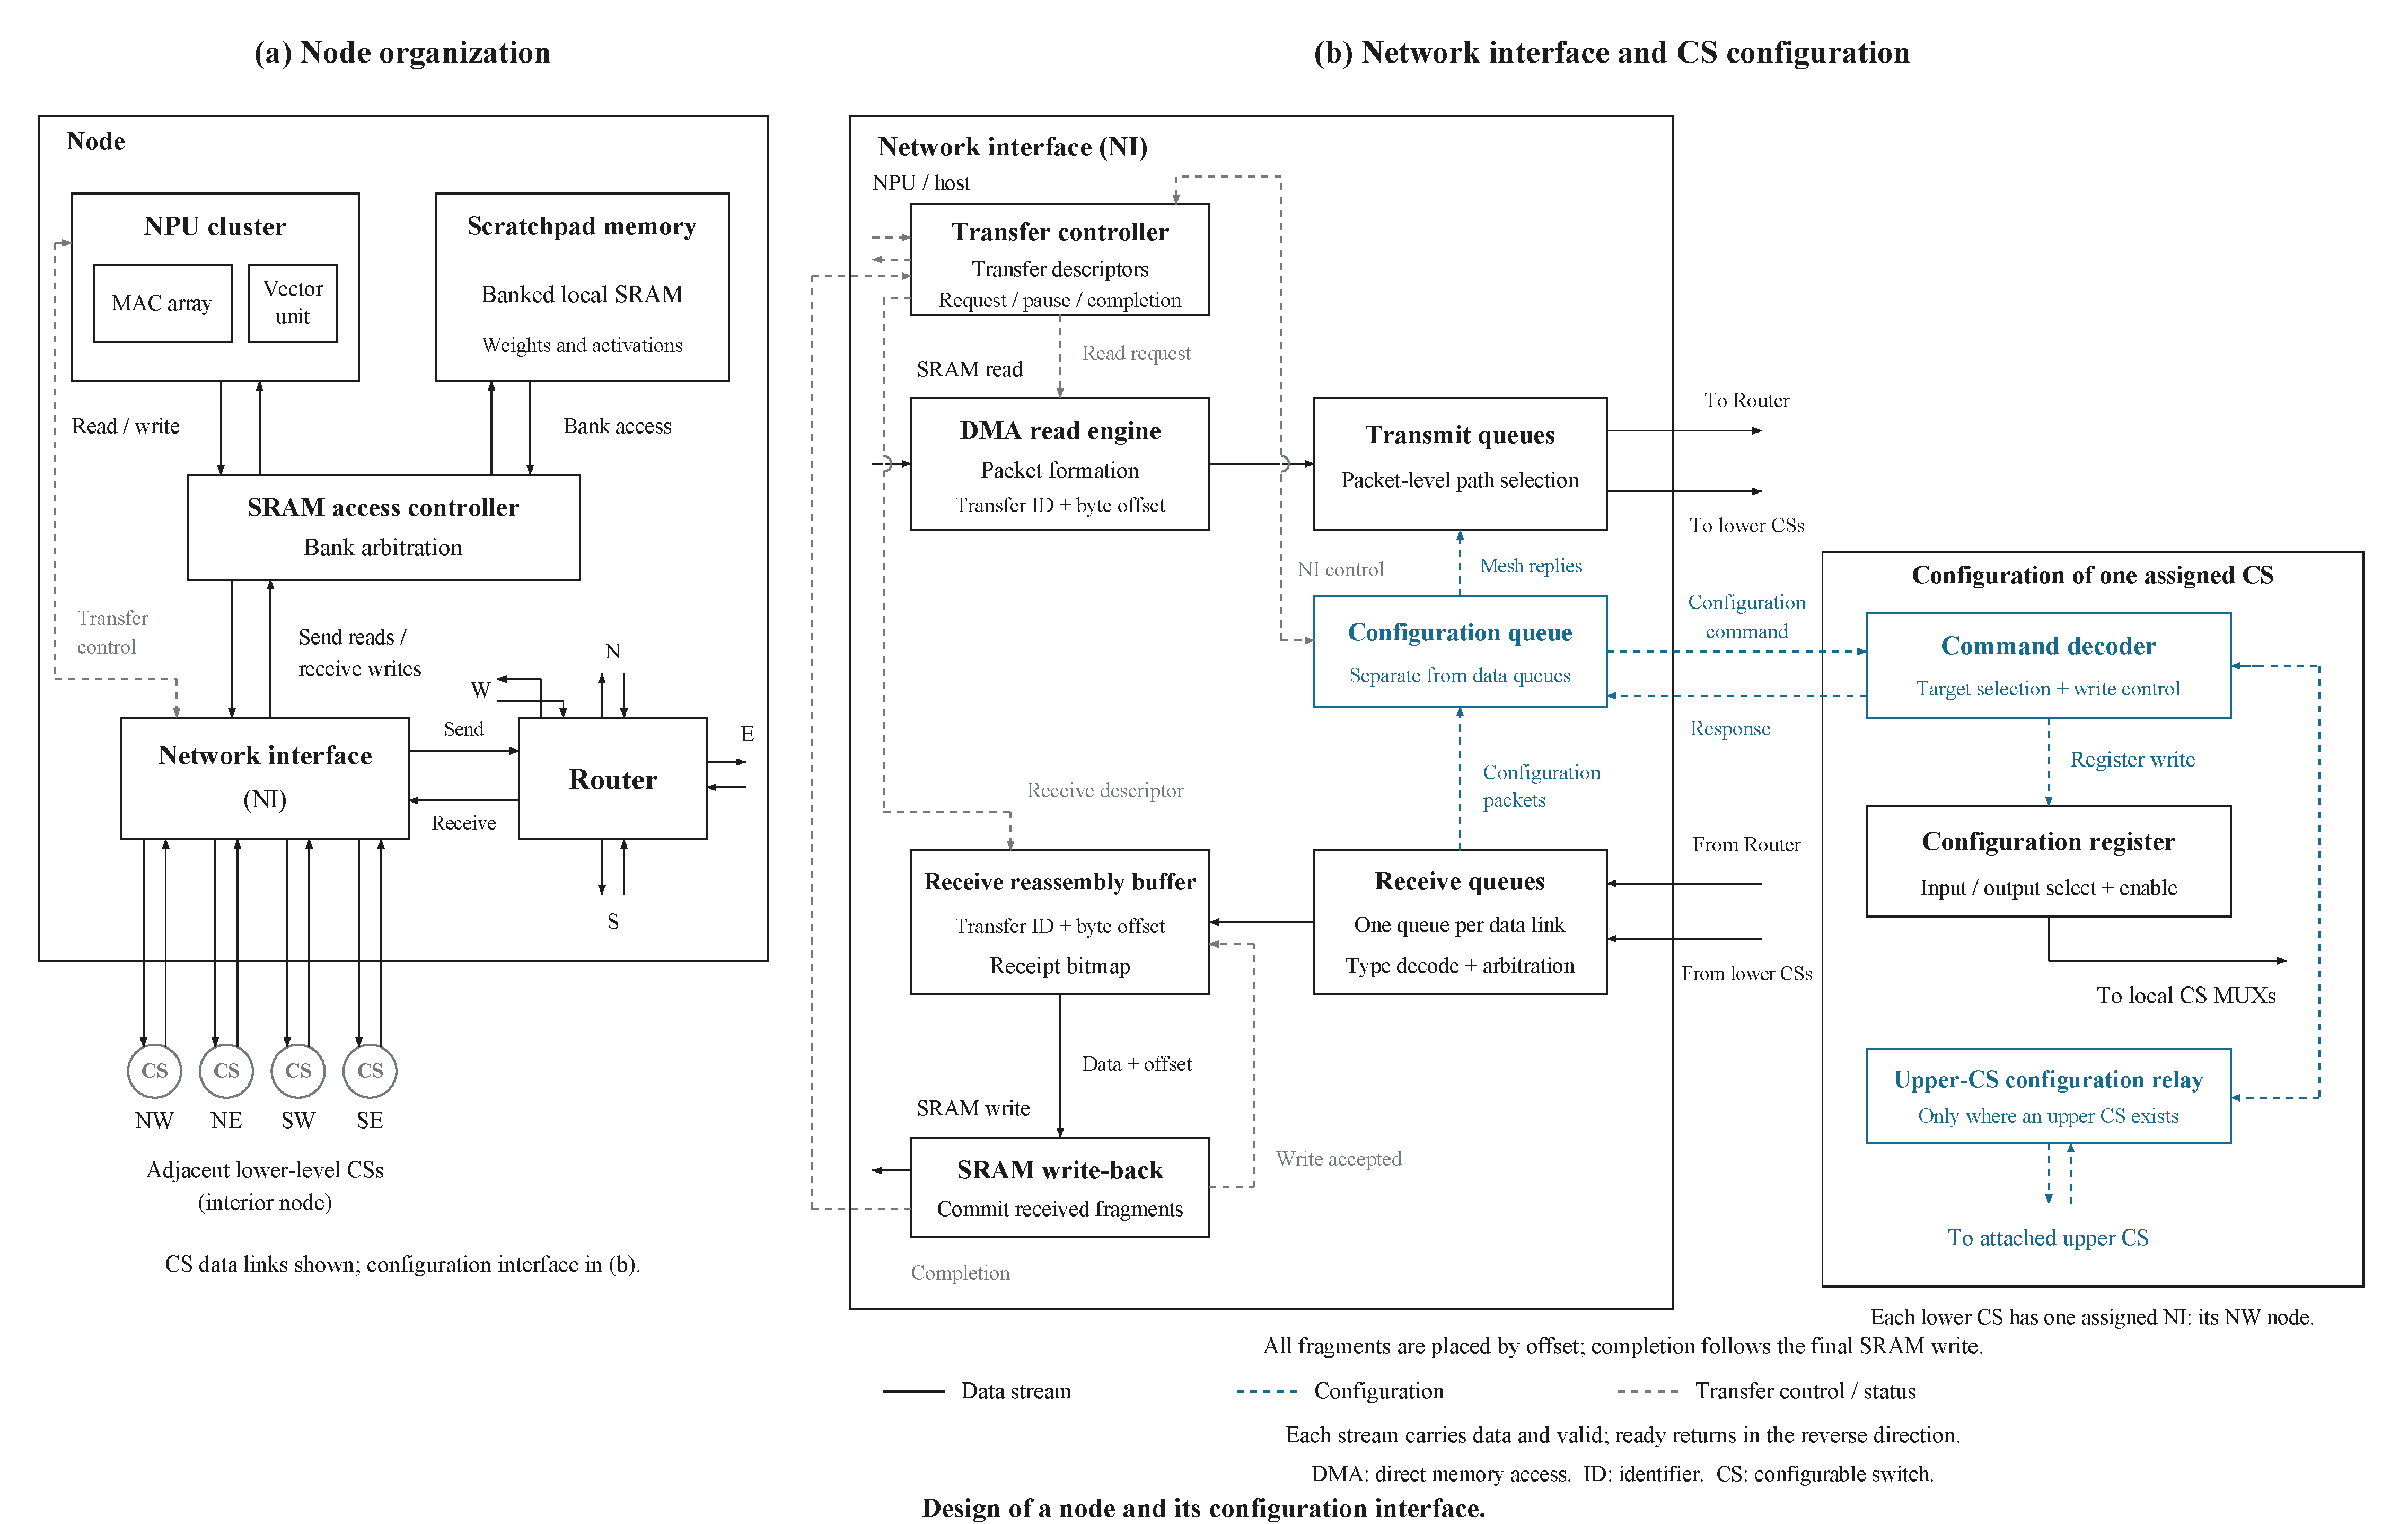
\includegraphics[width=\textwidth]{figures/noc_node_ni.pdf}
  \caption{Node and NI organization.
  (a) NPU, scratchpad, NI, Mesh router, and adjacent lower-CS data
  connections. (b) NI transmit, receive, and reassembly paths, together
  with the configuration interface of one assigned CS.
  Each lower CS is configured by its northwest node's NI.}
  \Description{A node contains an NPU cluster, local SRAM, shared bank
  arbitration, a network interface, and a Mesh router. The NI has separate
  adjacent-CS data streams. The expanded NI shows transfer control,
  packet formation, finite receive queues, offset-based reassembly,
  SRAM write-back, and a separate configuration queue. A CS-side decoder
  writes the configuration register and relays commands to an attached
  upper CS where present.}
  \label{fig:noc-node}
\end{figure*}

Figure~\ref{fig:noc-node}(b) shows the NI data path. The transfer controller
receives descriptors specifying the source and destination nodes, SRAM
addresses, transfer length, packet-to-CS assignments, and the
configuration version under which those attachments are usable.
A direct memory access (DMA) read engine
fetches source data and forms packets using the NI's configured payload
size. The final packet carries the remaining bytes. The sending and
receiving NIs use the same payload-size setting for a transfer.
Transmit queues select the Mesh or an assigned CS circuit for each complete packet.
A transfer may use several paths across its packets; the flits within
one packet follow the same path.
Each incoming data connection has a finite receive queue. Receive
arbitration feeds the reassembly buffer, while packet-type decoding
separates configuration commands from data.
CS streams carry data and a valid indication forward, with a ready
indication returning along the selected path. A transfer occurs when
valid and ready are both asserted.

Each data packet identifies its transfer by \texttt{TransferID}, formed
from the source NI and a source-local sequence number.
\texttt{Offset} gives its byte position within the transfer, and
\texttt{Length} gives the total transfer size. Receive descriptors
associate a transfer with its destination SRAM base address.
The NI derives each packet's index and expected payload length from
its offset, the transfer length, and the agreed payload size. It checks
the transfer identifier, offset alignment, and payload length before
writing the payload to the base address plus \texttt{Offset}.
A receipt bitmap has one bit per expected packet, updated after the
SRAM accepts that packet's payload write; already-received packets are
identified by their set bits. Transfers are admitted after allocating
their receive descriptors and bitmap storage.
Payloads can be written in arrival order while their offsets restore
the destination data layout.
The NI reports completion after all expected packet writes have completed;
the NPU then consumes the assembled data. This permits bounded
receive staging without holding later fragments until earlier ones
arrive. Reassembly writes and NPU accesses share the SRAM bank arbiter.

\subsection{Traffic Prediction}
\label{sec:traffic-prediction}

GetS requests and DataS responses use XY routing on plane C. The host
optimizes MoE routes on plane M. For Dispatch, we adapt MixNet's
adjacent-layer predictor~\cite{liao2025mixnet}:
\begin{equation}
  \widehat{\mathbf y}_{\ell,s}=P_\ell\mathbf x_{\ell-1,s},
  \quad P_\ell\geq0,\quad
  \mathbf1^{\mathsf T}P_\ell=\mathbf1^{\mathsf T}.
  \label{eq:noc-load-prediction}
\end{equation}
Here $\mathbf x_{\ell-1,s}$ is the preceding layer's normalized expert distribution
for tokens with known source NI $s$. Weighted least squares fits $P_\ell$
from paired token groups, weighting their size and recency. Prefill and
decode use separate models, with a historical-mean fallback.
Expert placement and packing map forecasts to source--destination
demand. Final allocation uses actual Top-K and packing metadata.
Combine uses confirmed assignments, output shapes, and estimated
expert completion times to derive return packets and release times.

\subsection{Reconfiguration Problem}
\label{sec:noc-problem}

Within a fixed $H$-cycle planning interval, $\mathcal M_f$ contains
the unbound packets of MoE source--destination flow $f$.
Their payloads $b_m$ give $D_f=\sum_{m\in\mathcal M_f}b_m$ and
$\mathcal M=\bigcup_f\mathcal M_f$. Legal CS paths for packet $m$
form $\mathcal P_m$, with $\mathcal P=\bigcup_m\mathcal P_m$.
Each simple path connects the source and destination NI through wired
CS ports. Binary $z_p$ selects path $p$;
binary $x_{m,p}$ assigns packet $m$ to it. We maximize useful payload
assigned to the CS network:
\begin{equation}
  \max_{\mathbf z,\mathbf x}\quad
  V=\sum_{m\in\mathcal M}b_m\sum_{p\in\mathcal P_m}x_{m,p}.
  \label{eq:noc-volume-objective}
\end{equation}
Readiness flag $g_m$ equals one when source data and receive storage
are ready, and zero otherwise. Each packet uses at most one enabled path:
\begin{equation}
  \sum_{p\in\mathcal P_m}x_{m,p}\leq1,
  \qquad x_{m,p}\leq z_p,\quad x_{m,p}\leq g_m.
  \label{eq:noc-packet-assignment}
\end{equation}
Selected paths are CS-disjoint. With $A_{c,p}=1$ when $p$ uses CS $c$,
\begin{equation}
  \sum_{p\in\mathcal P}A_{c,p}z_p\leq1,
  \qquad c=0,\ldots,12.
  \label{eq:noc-cs-exclusion}
\end{equation}

Resource $r\in\mathcal R$ is an M-plane link or NI, DMA, or SRAM service.
Its remaining budget $C_r$ within $H$ deducts work outside $\mathcal M$:
existing transfers, configuration messages, and C-plane use of shared endpoints.
Cost $u_{m,p,r}$ includes framing and expresses service in NoC cycles.
Unassigned packets use the M-plane Mesh, denoted
by 0, with $x_{m,0}=1-\sum_{p\in\mathcal P_m}x_{m,p}$. Thus,
\begin{equation}
  \sum_{m\in\mathcal M}\sum_{p\in\mathcal P_m\cup\{0\}}
  u_{m,p,r}x_{m,p}\leq C_r,\qquad r\in\mathcal R.
  \label{eq:noc-resource-capacity}
\end{equation}
At most two paths are selected, $\sum_{p\in\mathcal P}z_p\leq2$;
a path may traverse multiple CSs.
Path $p$ specifies the input, output, and enable fields of each CS;
$x_{m,p}$ determines the source NI's route tag for packet $m$.

\subsection{Configuration Algorithm}
\label{sec:noc-algorithm}

Offline enumeration supplies local and upper-CS paths. We target the two
M-plane links with the largest pending MoE flit counts. For each link
still unrelieved, flows are visited in decreasing $D_f$, with endpoint
identifiers breaking ties. Up to $K_p=2$ paths per flow are tried by length
and then identifier. We retain the first CS-disjoint extension that passes
joint \textsc{Assign} and increases $V$. Construction ends after two paths,
both links, or budget exhaustion. At most two configurations are retained;
the one-path configuration remains available when a second path is added.

Candidates are checked in decreasing $V$. A timing model propagates
source reads, finite queues, credits, receive writes, and dependencies;
DataS follows its request's memory service. While $S_0$ forwards, an update
must satisfy, using the same time origin,
\begin{equation}
  \widehat T(S)+\eta(S)<\widehat T(S_0).
  \label{eq:noc-switching-check}
\end{equation}
Here $\eta(S)\geq0$ is calibrated from paired errors on held-out requests.
Protected consumers satisfy
$\widehat T_k(S)-\widehat T_k(S_0)+\eta_k(S)\leq\epsilon_k$,
including MoE with $\epsilon_k=0$ and coherence transactions with their
specified allowances. Estimates include controller execution, pause,
drain, writes, and NI installation. After pause acknowledgement and drain, versions and eligibility are refreshed and feasibility, timing, and budgets are
rechecked before Section~\ref{sec:noc-config-interface}'s update protocol.

\begin{algorithm}[H]
  \caption{CS configuration for at most two hotspots}
  \label{alg:noc-configuration}
  \small
  \begin{algorithmic}[1]
    \Require MoE packets $\mathcal M$, paths $\mathcal P$, budgets $C_r$, active $S_0$
    \Ensure $S_0$, an acknowledged update, or an update error
    \State $\mathcal H\gets$ up to two M-plane links with largest demand
    \State $S\gets$ Mesh allocation; $\mathcal C\gets\varnothing$
    \For{$e\in\mathcal H$ while construction budget remains}
      \State \textbf{if} $S$ already relieves $e$ \textbf{then continue}
      \State $S'\gets$ first feasible extension for $e$ increasing $V$, or $S$
      \If{$V(S')>V(S)$}
        \State $S\gets S'$; $\mathcal C\gets\mathcal C\cup\{S\}$
      \EndIf
      \State \textbf{if} two paths are selected \textbf{then break}
    \EndFor
    \For{$S'\in\mathcal C$ in decreasing $V$}
      \State \textbf{if} budget expired \textbf{then return} $S_0$
      \State Estimate completion and update overhead
      \If{timing checks pass within the decision budget}
        \State Request packet holds and pause new CS admissions
        \If{pause and drain complete within budget}
          \State Refresh state; recheck feasibility and timing
          \State \textbf{if} final checks pass \textbf{then return} $\Call{ApplyCS}{S'}$
        \EndIf
        \State Release holds and resume $S_0$; \Return $S_0$
      \EndIf
    \EndFor
    \State \Return $S_0$
  \end{algorithmic}
\end{algorithm}


\subsection{Configuration Interface}
\label{sec:noc-config-interface}

The host CPU sends configuration packets over the ordinary Mesh to the
NI assigned to the target CS. Each lower CS is assigned to the NI of
its northwest corner node. This fixes one configuration writer per CS,
independently of its four neighboring data connections.
The NI places commands in a separate configuration queue and sends them
through a local command/response interface to the CS-side configurator.
The NI serializes writes to each assigned CS and rejects obsolete
configuration versions before forwarding commands.
The CS-side command decoder acts as the configurator: it decodes the
target and operation, writes the CS configuration register, and returns
a response.
For an upper CS, the corresponding lower CS relays the command and
response over a fixed inter-level control interface.
These local control interfaces operate independently of the CS data
MUX settings. Responses return through the NI and ordinary Mesh.

Table~\ref{tab:noc-command-fields} defines the packet and command fields.
A CS state is $q_c=(s_c^{\mathrm{out}},s_c^{\mathrm{in}},e_c)$, where
$c\in\{0,\ldots,12\}$ identifies the target CS,
$s_c^{\mathrm{out}}$ selects its output direction,
$s_c^{\mathrm{in}}$ selects an allowed input at that output's MUX,
and $e_c$ enables the connection.
The lower CS uses three output bits, two input bits, and one enable bit;
the upper CS uses two output bits, one input bit, and one enable bit.
Lower output codes 000--100 select NW, NE, SW, SE, and U, respectively.
Upper codes 00, 01, and 10 select the instance's horizontal direction,
vertical in-plane direction, and D. Input codes follow the remaining
input order shown at each MUX. A cleared enable or an unused output
code disables the connection.

\begin{table}[!t]
  \caption{Configuration packet and command fields.}
  \label{tab:noc-command-fields}
  \centering
  \small
  \begin{tabularx}{\columnwidth}{@{}p{0.25\columnwidth}>{\raggedright\arraybackslash}X@{}}
    \hline
    Field & Meaning \\
    \hline
    Type & Distinguishes configuration commands, responses, and data. \\
    Destination & Mesh destination NI assigned to the target. \\
    TransactionID & Matches a request to its response. \\
    ConfigVersion & Identifies the CS image and matching NI assignments. \\
    Target & CS index $c$, or transfer identifier for NI descriptor installation. \\
    Operation & CS write, NI descriptor installation, pause, status, or resume. \\
    State & CS tuple $q_c$, or NI packet-to-CS assignments indexed by byte offset. \\
    Status & Completion or failure reported in a response. \\
    \hline
  \end{tabularx}
\end{table}

The response echoes \texttt{TransactionID}, \texttt{Target}, and
\texttt{ConfigVersion};
an upper-CS write is acknowledged after the upper register accepts it.
The NI handles its own pause, status, and resume commands locally.
They control transfer admission and completion reporting, while
CS-targeted commands go to the CS-side configurator.
NI descriptor-installation commands associate a transfer identifier
with its packet-to-CS assignments and configuration version.
Each assigned packet is identified by its byte offset; its source-CS
attachment is stored as a route tag in the transmit queue. Packets
without such an assignment use the Mesh.
The transfer controller acknowledges installation after storing the
descriptor and confirming the required receive context. Its version
must match the applied configuration before CS admission.

To change the network, the host first pauses admission of new CS
transfers at all NIs. Previously admitted transfers finish transmission,
reassembly, and SRAM write-back. The host collects their drain responses
over the Mesh, writes the new CS states, and waits for every target's
write response. It then installs the matching NI descriptors and waits
for their acknowledgements before resuming admission.
A failed or incomplete update
keeps CS transmission paused. This sequence prevents data from
traversing a partially updated circuit.

\subsection{Thermal-Aware Execution}
\label{sec:thermal-design}

Thermal-aware execution complements bank placement and
NoC reconfiguration by adjusting operator frequencies and
task start times to reduce latency under thermal constraints.
Let $s_j$ and $r_j$ denote the start time and frequency
ratio of task $j$. The execution objective is
\begin{equation}
\begin{aligned}
  \min_{\{s_j,r_j\}} \quad & T_{\mathrm{inf}} \\
  \mathrm{s.t.}\quad
  & T_b[k]\leq T_{\mathrm{limit}},\quad \forall b,k,
\end{aligned}
\label{eq:thermal-optimization}
\end{equation}
where $T_{\mathrm{inf}}$ is the inference completion time
and $T_b[k]$ is the temperature of physical block $b$ at
thermal sampling step $k$.
We address this objective through offline operator-level
energy-aware DVFS and runtime thermal-aware task scheduling.


\noindent\textbf{Operator-Level Energy-Aware DVFS.}
We profile each operator type at three DVFS settings, $r\in\{1.0,0.75,0.5\}$, with separate profiles for different execution configurations. For each profile, we select the frequency that minimizes total execution energy, including dynamic and idle energy. For operators with overlapping computation and memory accesses, reducing the frequency can lower energy consumption with little increase in execution time. This can reduce heat generation and mitigate thermal throttling during inference.

\noindent\textbf{Model-Based Thermal Scheduling.}
We use a HotSpot-based RC thermal model~\cite{hotspot_tool} to capture delayed heat propagation between the Logic and DRAM tiers. Rather than repeatedly performing full RC simulations during scheduling, we precompute the temperature responses of individual tasks, including delayed temperature peaks after task completion. At runtime, the controller evaluates the predicted temperatures of candidate tasks and selects the task with the earliest feasible start time.

\FloatBarrier

\section{Evaluation Results and Analysis}
\label{sec:experiment}

\subsection{Experimental Setup}

We evaluate the proposed design on a face-to-face hybrid-bonded 3D accelerator. Table~\ref{tab:eval-platform} lists the common platform parameters. The evaluation uses 32~GiB of HB-DRAM. Each comparison starts from the same input and initial system state and uses the same precision, resource budget, and workload completion criteria. We account for each method's additional hardware and runtime costs separately.

\begin{table}[t]
\caption{Common hardware and simulation settings.}
\label{tab:eval-platform}
\centering\small
\begin{tabular}{@{}lp{0.59\columnwidth}@{}}
\hline
Component & Configuration \\
\hline
Logic tier & 16 NPU clusters at 1~GHz \\
NPU cluster & 4096 MACs, 16-lane vector unit, 4~MiB SRAM \\
Base NoC & $4\times4$ mesh, 256-bit links at 1~GHz \\
HB-DRAM & 32~GiB, 16 partitions of 2~GiB each, 16 logical banks per partition \\
Vertical link & 25.6~GB/s per NPU--memory pair \\
Host & Four CPU cores, PCIe 5.0, host memory xxx \\
Simulation & Compute, memory, and NoC models xxx \\
Thermal model & Ambient and initial temperatures xxx, temperature limit xxx \\
\hline
\end{tabular}
\end{table}

Table~\ref{tab:eval-workloads} lists four main MoE workloads and one auxiliary thermal scenario. We freeze the input manifests, arrival order, seeds, and stopping rules before collecting performance results. In each run of the main co-execution evaluation, we release a batch of synthetic coherence requests representing a general-purpose task before starting the MoE workload, so that the two traffic streams overlap. We use the same release schedule for HiBand and the proposed design.

\begin{table*}[t]
\caption{Workloads, input manifests, and measurement boundaries.}
\label{tab:eval-workloads}
\centering\small
\begin{tabularx}{\textwidth}{@{}p{0.25\textwidth}Xp{0.29\textwidth}@{}}
\hline
Workload & Inputs and configuration & Measurement boundary \\
\hline
Qwen3-30B-A3B & Prompt source and IDs xxx, input/output lengths xxx, concurrency xxx & Prefill, decode, and complete request \\
Qwen1.5-MoE-A2.7B & Prompt source and IDs xxx, lengths xxx, TP/PP mapping xxx & Prefill, decode, and complete request \\
mini-SWE-agent + Qwen3 & SWE-bench Lite instance IDs and split xxx, tool and stopping rules xxx & Model calls, full agent task, and task outcome \\
LingBot TI2V & Text/image IDs xxx, resolution xxx, frames xxx, steps and seeds xxx & Encoding, denoising, scheduler, and VAE decoding \\
WHISPER + SLAM + $\pi_{0.5}$ & WHISPER version xxx, SLAM and $\pi_{0.5}$ traces xxx, request schedule xxx & Joint thermal scenario, execution coverage xxx \\
\hline
\end{tabularx}
\end{table*}

For each experimental line, we first run the complete workload under both configurations and record stage latencies and the end-to-end critical path. Subsequent paired points measure the same one or two MoE layers with identical input and routing samples. We extrapolate both arms using the same layer selection, weights, and dependency model, including non-MoE stages and control costs. Recomputing the critical path preserves overlap among compute, memory, and communication. We validate the estimates against the complete runs and report measured layer latency, estimated end-to-end latency, and estimated speedup separately. The corresponding estimation errors are xxx. All reported execution times refer to the modeled target system.

\subsection{End-to-End Performance Comparison}

The primary comparison pairs the common platform baseline B with B plus the full design. We separately compare with prior methods that pass the same workload and timing checks under matched resource constraints. The HiBand reference implementation and other candidate NoCs enter this comparison after qualification. Table~\ref{tab:eval-comparisons} records the scope of each comparison.

\begin{table}[t]
\caption{Configurations and scope of the performance comparisons.}
\label{tab:eval-comparisons}
\centering\small
\begin{tabular}{@{}lp{0.53\columnwidth}@{}}
\hline
Configuration & Comparison scope \\
\hline
B & Common platform baseline, frozen configuration xxx \\
B + full design & Paired end-to-end comparison with B \\
HiBand reference & External comparison, qualification pending \\
Other NoC candidates & Configurations and qualification results xxx \\
\hline
\end{tabular}
\end{table}

Figure~\ref{fig:eval-overall} compares completion times for each main workload. For each pair, we compute the latency reduction as $1-T_{\mathrm{design}}/T_{\mathrm{ref}}$, where $T_{\mathrm{ref}}$ is the completion time of B or the named external comparator. We also report time to first token and time per output token for the language-model workloads. For mini-SWE-agent, we report model-call latency and task latency separately and record task outcomes. For LingBot, we report the latency of a complete generation. The measured end-to-end latencies, paired reductions, and workload-level exceptions are xxx.

\begin{figure*}[t]
\centering
\fbox{\rule{0pt}{18mm}\rule{0.92\textwidth}{0pt}}
\caption{End-to-end latency by workload for B, B plus the full design, and qualified external comparators. Each panel uses identical inputs and completion criteria. Labels distinguish complete-run measurements from estimates based on sampled MoE layers.}
\Description{Reserved space for the end-to-end latency comparison.}
\label{fig:eval-overall}
\end{figure*}

\subsection{Supporting Results and Thermal Ablation}

\paragraph{Phase-dependent congestion and bank waiting.}
To explain the latency differences in Figure~\ref{fig:eval-overall}, we trace matched MoE communication phases from memory requests through consumer readiness. We measure bank queueing before data becomes available, injection and router queueing, unloaded traversal, and synchronization at the slowest endpoint. We record configuration delay on the same timeline and attribute only exposed delays to the critical path. Comparing packet tails and router activity across phases tests whether a change in hotspot location translates into earlier consumer readiness. A comparison with fixed network policy and a bank-policy toggle can isolate the incremental effect of bank conflict mitigation. The paired changes in exposed waiting and packet tail latency are xxx.

\begin{figure*}[t]
\centering
\fbox{\rule{0pt}{17mm}\rule{0.92\textwidth}{0pt}}
\caption{Critical-path latency breakdown for matched MoE communication phases. The timeline shows bank service, data readiness, NoC injection and queueing, configuration, and consumer synchronization. Companion panels show packet tail latency and router activity using common scales across configurations.}
\Description{Reserved space for the critical-path breakdown and congestion panels.}
\label{fig:eval-breakdown}
\end{figure*}

\paragraph{Incremental effect of thermal management.}
We compare NoC with bank conflict mitigation and thermal management against the same NoC and bank mechanisms with thermal management disabled. Both arms start with identical temperatures, inputs, and thermal constraints. We track temperatures over the complete execution timeline and account for DVFS adjustments and thermal-aware task scheduling. We report natural and thermally stressed scenarios separately. Peak temperature, time above the threshold, and completion time are xxx.

\begin{figure}[t]
\centering
\fbox{\rule{0pt}{17mm}\rule{0.90\columnwidth}{0pt}}
\caption{Temperature and workload progress under different thermal management strategies. All configurations use the same NoC and DRAM-bank policies. }
\Description{Reserved space for temperature and workload progress curves.}
\label{fig:eval-thermal}
\end{figure}

\subsection{Scalability and Sensitivity Analysis}

We vary system scale and input scale separately. The system-scale sweep starts at 16 NPU clusters and holds workload fixed. At each scale, we report the topology, mapping, capacity, and bandwidth. The input-scale sweep fixes the platform and varies request concurrency or input size. We report absolute completion time and paired latency reduction at each point. To examine design sensitivity, we vary the local connection budget and reconfiguration interval one at a time and record completion time, packet tail latency, and exposed configuration cost. The tested ranges and observed trends are xxx.

\begin{figure}[t]
\centering
\fbox{\rule{0pt}{17mm}\rule{0.90\columnwidth}{0pt}}
\caption{Scalability and sensitivity. Panels show (a) system scale at fixed workload, (b) input scale at fixed system size, and (c) sensitivity to the local connection budget and reconfiguration interval. Markers indicate the default configuration and whether overall latency is measured or estimated.}
\Description{Reserved space for the scalability and parameter sweeps.}
\label{fig:eval-scale}
\end{figure}

\subsection{Hardware Cost and Runtime Overhead}

Table~\ref{tab:eval-cost} compares a fixed $4\times4$ mesh with 256-bit links against the same mesh augmented by 13 circuit switches (CSs). The NoC prototypes use simplified network interfaces and exclude SRAM bank control, thermal control, and physical cross-tier links. Each pair uses the same tools and constraints. The 1\,GHz NoC clock in Table~\ref{tab:eval-platform} is a system simulation parameter.

Directed RTL tests cover all 256 mesh source--destination pairs, 108 lower-tier CS paths, and 24 directed upper-tier routes. The tests also check that the controller rejects cyclic configurations and waits for circuits to drain under backpressure before committing a new configuration.

\begin{table}[t]
\caption{Hardware implementation cost of the two NoC prototypes.}
\label{tab:eval-cost}
\centering\small
\begin{tabular}{@{}lrr@{}}
\hline
Metric & Fixed mesh & Mesh + 13 CSs \\
\hline
\multicolumn{3}{@{}l@{}}{\textit{FPGA post-route (200\,MHz constraint)}} \\
LUTs & 26,893 & 37,441 \\
Flip-flops & 21,025 & 24,451 \\
BRAM / DSP & 0 / 0 & 0 / 0 \\
Setup WNS (ns) & $+0.528$ & $+0.290$ \\
\hline
\multicolumn{3}{@{}l@{}}{\textit{ASIC synthesis}} \\
Std. cell area ($\mathrm{mm}^{2}$) & 0.205446 & 0.250919 \\
Total power (W) & 1.46 & 1.65 \\
\hline
\multicolumn{3}{@{}l@{}}{\textit{ASIC post-route}} \\
Std. cell area ($\mathrm{mm}^{2}$) & 0.359453 & 0.458480 \\
Dynamic power (W) & 0.661 & 0.721 \\
Leakage power (mW) & 11.7 & 15.2 \\
\hline
\end{tabular}
\par\smallskip
\begin{minipage}{\columnwidth}
\footnotesize
FPGA results use Vivado 2017.4 on \texttt{xcku5p-ffva676-2-e}.
Setup WNS is from out-of-context post-route static timing analysis with a 5\,ns clock constraint.
ASIC results use Nangate45 TT (1.10\,V, $25\,^{\circ}\mathrm{C}$).
ASIC power estimates use a 1\,ns clock constraint, vectorless activity 0.10, and duty cycle 0.50. Post-route power estimates include OpenRCX SPEF parasitics.
\end{minipage}
\end{table}

Relative to the fixed mesh, the enhanced prototype uses 39.2\% more LUTs and 16.3\% more flip-flops after FPGA routing. The routed ASIC uses 27.5\% more standard-cell area and 9.1\% more estimated dynamic power under the same power assumptions.

Table~\ref{tab:eval-runtime} reports algorithm execution separately from the delay of applying its decisions. For each algorithm, we measure per-call time and call count, then report the fraction of total application latency exposed on the critical path. Configuration transfer, hardware reconfiguration, and thermal scheduling overhead are accounted for as separate events.

\begin{table}[t]
\caption{Runtime overhead of online decision algorithms.}
\label{tab:eval-runtime}
\centering\small
\begin{tabular}{@{}lccc@{}}
\hline
Algorithm & Time/call & Calls & Exposed share \\
\hline
Hotspot prediction & xxx & xxx & xxx \\
Connection selection & xxx & xxx & xxx \\
Bank policy & xxx & xxx & xxx \\
Thermal control & xxx & xxx & xxx \\
\hline
\end{tabular}
\end{table}

\section{Related Works}
\label{sec:related-works}

\section{Conclusion}
\label{sec:conclusion}

\bibliographystyle{IEEEtran}
\bibliography{references,thermal_references}

\end{document}

